\documentclass[10pt,a4paper]{article}

% ---------------------------------------------------------------------------
% AgentM2M explained: a step-by-step walkthrough on DevBench `chakin`.
% Companion to docs/DS-A2A.tex. Every "engine output" listing below was
% produced by running the real prototype (src/agentm2m) on the DevBench
% `chakin` repository; LLM answers are either copied from the logged
% qwen3-coder:30b pilot run (evaluation/harness/logs/*qwen3-coder-30b*) or
% scripted to match them, so that keys, stamps and reports are reproducible.
% ---------------------------------------------------------------------------

\usepackage[T1]{fontenc}
\usepackage[utf8]{inputenc}
\usepackage{lmodern}
\usepackage[margin=2.3cm]{geometry}
\usepackage{amsmath,amssymb,amsthm}
\usepackage{booktabs,multirow,array,tabularx}
\usepackage{xcolor}
\usepackage{enumitem}
\usepackage{listings}
\usepackage{tikz}
\usepackage{graphicx}
\graphicspath{{../evaluation/results/figures/}}
\usetikzlibrary{arrows.meta,positioning,shapes.geometric,fit,backgrounds,calc}
\usepackage{pifont}
\usepackage[strings]{underscore} % plain _ in \texttt identifiers
\usepackage[hidelinks]{hyperref}
\usepackage{cleveref}

\newcommand{\cmark}{\ding{51}}
\newcommand{\xmark}{\ding{55}}
\newcommand{\pmark}{\ding{109}}

% --- shorthands (same as the paper) ---
\newcommand{\tool}{\textsc{AgentM2M}}
\newcommand{\devteam}{\textsc{DevTeam}}
\newcommand{\MM}{\mathit{MM}}
\newcommand{\Mods}[1]{\mathcal{M}(#1)}
\newcommand{\TL}{\mathit{TL}}
\newcommand{\team}{\mathcal{T}}
\newcommand{\str}{\mathrm{str}}
\newcommand{\sem}{\mathrm{sem}}
\newcommand{\Dist}[1]{\mathcal{D}(#1)}
\newcommand{\fp}{\mathit{fp}}
\newcommand{\Obl}{\mathit{Obl}}
\newcommand{\cls}[1]{\textsf{#1}}
\newcommand{\code}[1]{\texttt{#1}}
\newcommand{\file}[1]{\texttt{#1}}
% robust: \tikz inside a caption (a moving argument) breaks otherwise
\DeclareRobustCommand{\tracemark}{\tikz[baseline=-0.6ex]\node[draw,diamond,fill=black!70,inner sep=1.1pt]{};}

% --- listing styles ---
\definecolor{rawbg}{RGB}{255,248,230}
\definecolor{modelbg}{RGB}{235,244,255}
\definecolor{enginebg}{RGB}{236,250,238}
\definecolor{llmbg}{RGB}{248,238,252}

\lstdefinelanguage{ATL}{
  morekeywords={module,create,from,rule,to,lazy,unique,helper,def,
                context,uses,thisModule,and,or,not,in},
  morekeywords=[2]{@llm,@check}, alsoletter={@},
  sensitive=true, morecomment=[l]{--}, morestring=[b]'}
\lstdefinelanguage{KM3}{
  morekeywords={package,class,attribute,reference,container,
                enumeration,literal,datatype,oppositeOf},
  sensitive=true, morecomment=[l]{--}}

\lstset{frame=single, basicstyle=\ttfamily\footnotesize, breaklines=true,
        breakatwhitespace=false, columns=fullflexible, keepspaces=true,
        showstringspaces=false, numbers=none, upquote=true,
        keywordstyle=\bfseries, keywordstyle={[2]\bfseries\color{purple}},
        commentstyle=\itshape\color{black!60},
        captionpos=t, aboveskip=6pt, belowskip=6pt,
        literate={->}{{$\rightarrow$}}2 {<-}{{$\leftarrow$}}2}
% "raw input" = what the benchmark / user / lead actually provides
\lstdefinestyle{raw}{backgroundcolor=\color{rawbg}, literate={}}
% "model" = a view model or metamodel as the engine holds it
\lstdefinestyle{model}{backgroundcolor=\color{modelbg}}
% "engine" = deterministic output of the AgentM2M runtime
\lstdefinestyle{engine}{backgroundcolor=\color{enginebg}, literate={}}
% "llm" = a prompt sent to / answer received from an LLM
\lstdefinestyle{llm}{backgroundcolor=\color{llmbg}, literate={}}

\crefname{lstlisting}{Listing}{Listings}
\Crefname{lstlisting}{Listing}{Listings}

\theoremstyle{definition}
\newtheorem{definition}{Definition}
\newtheorem{remark}{Remark}

% A small paragraph-style marker for the "what happens" narration.
\newcommand{\todo}[1]{\textcolor{red}{\textbf{[TODO: #1]}}}
\newcommand{\what}[1]{\par\smallskip\noindent\textbf{#1}\quad}

\title{\tool{} Explained:\\ A Step-by-Step Walkthrough on DevBench \texttt{chakin}}
\author{Companion document to ``\tool{}: M2M Transformations for Agentic
Collaborations in Software Engineering''}
\date{}

\begin{document}
\maketitle

\begin{abstract}
The \tool{} paper compresses its idea into a few pages: treat every hand-off
between LLM agents as an ATL-style model-to-model (M2M) transformation, let a
deterministic engine own the \emph{structure} of the hand-off, and confine the
LLM to validated \emph{stochastic bindings} that fill in attribute values from
a bounded source footprint. This companion document unpacks that idea on one
concrete input: the \texttt{chakin} repository from DevBench, the repository
used in the paper's pilot. For every step we show the \emph{raw input} (the
benchmark files, the user's or team lead's request, the LLM prompt) and then
explain what the engine does with it, one operation at a time. We cover how
each agent's ``language'' (its view metamodel) is defined and populated, how a
single hand-off runs, how a requirement change propagates, what happens when
several hand-offs fire at once, and what happens when a new agent joins the
team while it is running. All engine outputs shown were produced by running
the prototype on \texttt{chakin}.
\end{abstract}

\tableofcontents

% ===========================================================================
\section{How to read this document}\label{sec:read}
% ===========================================================================

The document follows the seven steps of the paper (Section~III) in order, but
each step is grounded in the \texttt{chakin} run. Listings are colour-coded by
where their content comes from:

\begin{center}
\small
\begin{tabular}{@{}l p{11.5cm}@{}}
\toprule
\colorbox{rawbg}{\strut\ Raw input\ } & Something the team receives from outside: a DevBench file (PRD, UML diagram, test configuration), a change request, a request from the team lead. \\
\colorbox{modelbg}{\strut\ Model\ } & A metamodel, a view model or a rule module, i.e., the ``language'' and the ``sentences'' agents exchange. \\
\colorbox{llmbg}{\strut\ LLM\ } & A prompt the engine sends to an LLM, or the value the LLM returns. \\
\colorbox{enginebg}{\strut\ Engine\ } & Deterministic output of the \tool{} runtime: trace links, version stamps, run reports, escalations. \\
\bottomrule
\end{tabular}
\end{center}

\paragraph{Where the numbers come from.} The final experiment, with two
models on 8 DevBench repositories, is described with all its tables and
figures in \Cref{sec:experiments}; the walkthrough sections before it use
\texttt{chakin} to explain each mechanism. The first pilot ran three
open-weight models on \texttt{chakin}. A review of those logs found two
implementation defects that inflated \tool{}'s LLM usage and hid the
criterion from the Developer (\Cref{sec:tokens}). Both are fixed, the old
logs are archived in \file{evaluation/harness/logs/archive\_pre\_fix/}, and
new runs write to \file{evaluation/harness/logs/devbench\_rq\{1,2,3\}\_<model>\_*.jsonl}.
Outputs quoted below that come from the \emph{pre-fix} run are labelled as
such; they are kept where they illustrate a mechanism or a defect. For this
document we re-ran the same code path
(\file{evaluation/harness/devbench_agentm2m_config.py},
\file{impact_injector_devbench.py}, \file{hot_reviewer_rq3.py}) with a scripted
LLM backend that returns the answers \texttt{qwen3-coder:30b} gave in the
logged run. This makes every trace key, stamp and report below exactly
reproducible. Where we quote a raw model answer that the scripted backend does
not reproduce (e.g., the full generated function bodies), we say so and quote
it from the log.

\paragraph{Prototype versus paper design.} The pilot instantiates the paper's
design with a few simplifications. They matter for understanding the results,
so we list them up front (\Cref{tab:diff}) and point them out again where they
show up.

\begin{table}[h]
\centering\small
\caption{Where the \texttt{chakin} pilot differs from the \devteam{} design in the paper.}
\label{tab:diff}
\begin{tabularx}{\textwidth}{@{}l X X@{}}
\toprule
Aspect & Paper design (\devteam{}) & \texttt{chakin} pilot (\file{devbench_rules/}) \\
\midrule
Hand-offs & $T_1$ Req2Arch, $T_2$ Arch2Code (reads Arch \emph{and} Req), $T_3$ Code2Test, $T_4$ Criterion2Test & Req2Arch, Arch2Code (reads Arch only), Req2Test; no Code2Test \\
Footprint of \code{body} & \code{op.signature} and the story's criteria (multi-source $T_2$) & \code{op.codeContext()}: signature plus the story's criteria, which Req2Arch copies \emph{structurally} into \code{op.spec} (single-source $T_2$, same information) \\
Guard on test cases & criterion's story must be \code{accepted} & no guard \\
Where $M_{\mathit{req}}$ comes from & \textsc{Lift} of the Analyst's text & deterministic parser over PRD + UML (\file{devbench_loader.py}) \\
Resample budget $k$ & free parameter & $k=2$ (\code{max_resamples=2}), at most 2 passes; an escalated binding is not re-sampled until its footprint changes \\
Scheduling of $D$ & worklist of readers of changed views & re-run all hand-offs in registration order until nothing changes \\
\bottomrule
\end{tabularx}
\end{table}

% ===========================================================================
\section{Background, made concrete}\label{sec:background}
% ===========================================================================

\subsection{The problem in one repository}

DevBench~\cite{li2024devbench} gives, for each repository, the documents a
software team would receive: a product requirements document (PRD), a UML
class diagram, a UML sequence diagram, an architecture design, and the real,
executable unit and acceptance tests the finished code is graded against.
\texttt{chakin} is a small Python library that searches and downloads
pre-trained word vectors. \Cref{lst:prd,lst:uml,lst:cfg} show the parts of
the raw input that matter for this walkthrough.

\begin{lstlisting}[style=raw, caption={Raw input 1: excerpt of \file{chakin/PRD.md}.}, label={lst:prd}]
## Features and Functionalities
- **Easy Installation**: `chakin` can be installed with a simple pip command.
- **Search Functionality**: Users can search for word vectors by language.
- **Download Functionality**: Users can download word vectors by specifying
  either a numerical index or a name.
- **Progress Tracking**: The download progress is visually tracked with a progress bar.
...
# Acceptance Criteria
- Feature complete as per the functionalities described above.
- Passing all unit tests included in the `test_downloader.py`.
\end{lstlisting}

\begin{lstlisting}[style=raw, caption={Raw input 2: \file{chakin/UML_class.md} (mermaid).}, label={lst:uml}]
classDiagram
    class Global_functions {
        <<global functions>>
        +load_datasets()
        +download(number: int, name: string, save_dir: string)
        +search(lang: string)
    }
    class TestDownloader {
        -name: string
        -number: int
        +test_download_by_name()
    }
    TestDownloader --> Global_functions : uses functions from
\end{lstlisting}

\begin{lstlisting}[style=raw, caption={Raw input 3: excerpt of \file{chakin/repo_config.json}.}, label={lst:cfg}]
"code_file_DAG": { "chakin/downloader.py": [] },
"unit_test_script": "pytest --cov=chakin ... unit_tests",
"acceptance_test_script": "python -m unittest acceptance_tests/acceptance_test.py",
\end{lstlisting}

A four-agent team (Analyst, Architect, Developer, Tester), organised by roles as in
MetaGPT or ChatDev~\cite{hong2024metagpt,qian2024chatdev}, has to turn these
documents into \file{chakin/downloader.py}. In a \emph{free-text} team, every
hand-off is a prose message that the next agent's LLM re-reads. The logged
free-text run of \texttt{qwen3-coder:30b} on \texttt{chakin} shows all three
deficits the paper identifies, using the MAST failure taxonomy~\cite{cemri2025mast}:

\begin{description}[leftmargin=1.2em, style=nextline]
\item[P1, lossy hand-offs.] The MAST annotator flagged FM-1.4 (loss of
conversation history) and FM-2.1 (conversation reset) in the transcript. No
information the Analyst received is structurally guaranteed to reach the
Developer.
\item[P2, no traceability under change.] When asked ``which operations need
re-implementing if the \code{load_datasets} criterion is tightened?'', the
free-text team answered \emph{all four} operations
(\code{download}, \code{load_datasets}, \code{search},
\code{test_download_by_name}); precision $0.25$. Nothing records which
artifact came from which requirement, so the only safe answer is ``redo
everything''.
\item[P3, structure lives in prompts.] Adding a security reviewer requires
editing the orchestration code: enumerate every existing operation, write a
new prompt, route the output (\Cref{sec:hot}).
\end{description}

\subsection{ATL in one page, on \texttt{chakin}}

\tool{} borrows its execution model from ATL~\cite{jouault2008atl}. The
vocabulary is summarised in \Cref{tab:glossary}; the rest of the document
uses each term on concrete data.

\begin{table}[h]
\centering\small
\caption{Vocabulary, each with its \texttt{chakin} instance.}
\label{tab:glossary}
\begin{tabularx}{\textwidth}{@{}l X X@{}}
\toprule
Term & Meaning & \texttt{chakin} instance \\
\midrule
Metamodel $\MM$ & The ``language'' of a view: classes, attributes, references. & \cls{Req}: \cls{Epic}, \cls{UserStory}, \cls{Criterion}. \\
Model $M\in\Mods{\MM}$ & A set of objects that \emph{conforms} to a metamodel. & $M_{\mathit{req}}$ with 2 epics, 9 stories, 9 criteria. \\
Matched rule & \code{from s : A!C (guard) to t : B!D (bindings)}: for every source \cls{C} that satisfies the guard, create one target \cls{D}. & \code{Story2Operation}: each accepted \cls{UserStory} yields one \cls{Operation}. \\
Match / match key & One tuple of source objects satisfying a rule's pattern and guard, identified by a stable key. & \code{s=UserStory\#Global_functions::download} \\
Trace link & Record (match, target, rule) created when a match is first seen. & Story \code{download} $\mapsto$ Operation \code{download} via \code{Story2Operation}. \\
Structural binding & A deterministic OCL expression that initialises a target feature. & \code{name <- s.id.realName()} \\
Resolution & A structural binding that yields a \emph{source} object is replaced by the \emph{target} object generated from it. & \code{component <- s.epic} yields the \cls{Component} made from that \cls{Epic}. \\
Stochastic binding & \code{f <- @llm(prompt, e)}: an LLM samples the value of attribute \code{f}, seeing only the footprint $e$. & \code{signature <- @llm('Derive...', s.criteria)} \\
Footprint $\fp_b(m)$ & The source data the expression $e$ reads for a match $m$. & The criterion object(s) of that one story. \\
Validator \code{@check} & A predicate the sampled value must pass before it is written. & \code{signature.parses()} \\
Version stamp & Digest of the footprint at the moment the value was accepted. & \code{79066a260a457952} \\
Obligation & A (target, binding) whose stamp no longer matches its footprint: it must be re-sampled. & (\code{Operation load_datasets}, \code{signature}) after a PRD edit. \\
Failed stamp & Digest of the footprint at the moment the binding was escalated; while it matches, the binding is not re-sampled (\Cref{sec:tokens}). & set for an oracle that failed \code{failsOnStub()} $k$ times \\
HOT & A transformation whose output is a transformation (here: a new hand-off plus team entries). & Adding \code{Arch2Sec} and a Security Reviewer mid-run. \\
\bottomrule
\end{tabularx}
\end{table}

ATL runs a module in two phases. \emph{Matching} evaluates every rule's source
pattern and guard on the read-only source model, creates one empty target
object per match and records a trace link. \emph{Initialisation} then
evaluates the bindings; when a binding yields a source object, ATL looks it up
in the trace and substitutes the target generated from it. Because sources
are read-only and every source object is matched by at most one rule, the
result does not depend on the order in which rules fire. \tool{} keeps this
execution model and adds one thing: some bindings are answered by an LLM, but
only after the structure is fixed and only for primitive attributes.

% ===========================================================================
\section{Overview of the \texttt{chakin} team}\label{sec:overview}
% ===========================================================================

\begin{figure}[h]
\centering
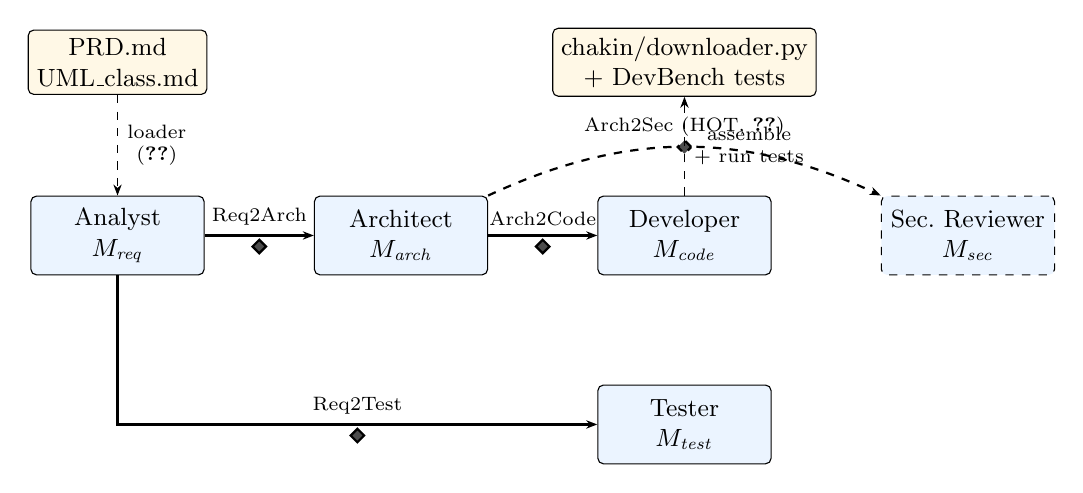
\begin{tikzpicture}[
  font=\small, >={Stealth[length=4pt]},
  raw/.style={draw, fill=rawbg, rounded corners=2pt, align=center, minimum height=8mm, inner sep=3pt},
  view/.style={draw, fill=modelbg, rounded corners=2pt, align=center, minimum width=22mm, minimum height=10mm, inner sep=3pt},
  tr/.style={->, thick},
  trace/.style={draw, diamond, fill=black!70, inner sep=1.3pt},
  lbl/.style={font=\scriptsize, align=center}]
  \node[raw] (prd) at (0,2.2) {PRD.md\\UML\_class.md};
  \node[view] (req)  at (0,0)    {Analyst\\$M_{\mathit{req}}$};
  \node[view] (arch) at (3.6,0)  {Architect\\$M_{\mathit{arch}}$};
  \node[view] (code) at (7.2,0)  {Developer\\$M_{\mathit{code}}$};
  \node[view] (test) at (7.2,-2.4) {Tester\\$M_{\mathit{test}}$};
  \node[view, dashed] (sec) at (10.8,0) {Sec.\ Reviewer\\$M_{\mathit{sec}}$};
  \node[raw] (out) at (7.2,2.2) {chakin/downloader.py\\+ DevBench tests};
  \draw[->, dashed] (prd) -- node[right, lbl] {loader\\(\Cref{sec:seed})} (req);
  \draw[tr] (req) -- node[above, lbl] {Req2Arch} node[below=1pt, trace] {} (arch);
  \draw[tr] (arch) -- node[above, lbl] {Arch2Code} node[below=1pt, trace] {} (code);
  \draw[tr] (req.south) |- node[pos=0.75, above, lbl] {Req2Test} node[pos=0.75, below=1pt, trace] {} (test.west);
  \draw[tr, dashed] (arch.north east) to[bend left=25] node[pos=0.5, above, lbl] {Arch2Sec (HOT, \Cref{sec:hot})} node[pos=0.5, trace] {} (sec.north west);
  \draw[->, dashed] (code) -- node[right, lbl] {assemble\\+ run tests} (out);
\end{tikzpicture}
\caption{The \texttt{chakin} pilot team. Solid arrows are the three hand-offs
registered at start-up; each keeps a persistent trace model
(\,\tracemark\,).
The dashed Security Reviewer and its hand-off \code{Arch2Sec} are added while
the team runs.}
\label{fig:overview}
\end{figure}

The end-to-end flow on \texttt{chakin} is:
\begin{enumerate}[nosep]
\item \textbf{Design time.} Define one metamodel per agent (Step~1,
\Cref{sec:step1}), the team model (Step~2, \Cref{sec:step2}) and the hand-off
rules (Step~3, \Cref{sec:step3}).
\item \textbf{Seeding.} Turn PRD + UML into the Analyst's model
$M_{\mathit{req}}$ (\Cref{sec:seed}).
\item \textbf{Runtime.} Run the hand-offs to a fixpoint (Step~4,
\Cref{sec:step4}), accept new text only through \textsc{Lift} (Step~5,
\Cref{sec:step5}), propagate changes through trace models (Step~6,
\Cref{sec:step6,sec:multi}), and let the engine decide when the team is done
(Step~7, \Cref{sec:step7}).
\item \textbf{Evolution.} Add a Security Reviewer with a higher-order
transformation (\Cref{sec:hot}).
\item \textbf{Grading.} Assemble the Developer's \cls{CodeEdit} bodies into
\file{chakin/downloader.py} and run DevBench's own tests.
\end{enumerate}

% ===========================================================================
\section{Step 1: Give every agent its own language (view metamodels)}\label{sec:step1}
% ===========================================================================

\subsection{Raw input: the role descriptions}

A view metamodel is written at design time from the team's role
descriptions. For \devteam{} the raw input is just the informal statement of
who produces what:

\begin{lstlisting}[style=raw, caption={Raw input 4: role descriptions (from the paper, Section~II-B).}, label={lst:roles}]
Analyst   : turns user requests into user stories grouped by epics,
            each with acceptance criteria.
Architect : designs components and API operations.
Developer : writes code edits.
Tester    : writes test cases with executable oracles and reports verdicts.
\end{lstlisting}

\subsection{What happens: from role description to metamodel}

A human (in the future, an ``architect agent'', see RC1 in the paper) reads
each role and asks three questions. We walk through them for the Analyst and
the Architect.

\what{Q1: What \emph{things} does this agent talk about?} Each noun that the
agent creates becomes a class. Analyst: \emph{epic}, \emph{user story},
\emph{acceptance criterion} $\Rightarrow$ \cls{Epic}, \cls{UserStory},
\cls{Criterion}. Architect: \emph{component}, \emph{operation}
$\Rightarrow$ \cls{Component}, \cls{Operation}.

\what{Q2: What does the agent say \emph{about} each thing?} Each property
becomes a primitive attribute. A story has an \code{id} and a
\code{status}; a criterion has an \code{id} and a \code{text}; an operation
has a \code{name} and a \code{signature}. Primitive attributes are
important: they are the \emph{only} features an LLM may ever fill
(\Cref{sec:step3}).

\what{Q3: How do the things relate?} Each relation becomes a reference.
``stories grouped by epics'' $\Rightarrow$ \code{UserStory.epic : Epic};
``each with acceptance criteria'' $\Rightarrow$ a \emph{containment}
reference \code{UserStory.criteria : Criterion[1..*]} (a criterion cannot
exist without its story); ``operations belong to components'' $\Rightarrow$
\code{Operation.component : Component}.

\what{What the agent does \emph{not} get.} The Architect's \cls{Operation}
has no reference to \cls{UserStory}, and the Analyst's metamodel knows
nothing about operations. Each view stays in its owner's terms, as in
view-based development~\cite{klare2021vitruvius,bruneliere2019views}. How a story
and an operation correspond is recorded later, by the hand-off, in a
separate trace model~\cite{jouault2005traceability,vara2014metagem}, not in either metamodel.

\subsection{Result: the four metamodels}

\Cref{lst:km3} shows the result in the paper's KM3-like notation;
\Cref{lst:pyecore} shows the same metamodel as the prototype actually builds
it (pyecore, i.e., EMF-compatible Ecore).

\begin{lstlisting}[language=KM3, style=model, caption={The four view metamodels of the pilot (KM3-like).}, label={lst:km3}]
package Req {                                   -- owned by Analyst
  class Epic      { attribute name : String; }
  class UserStory { attribute id : String;  attribute status : String;
                    reference epic : Epic;
                    reference criteria[1-*] container : Criterion; }
  class Criterion { attribute id : String;  attribute text : String; }
  class ModuleCriterion { attribute id, text : String; } -- held once, read by no footprint
}
package Arch {                                  -- owned by Architect
  class Component { attribute name : String; }
  class Operation { attribute id, name, signature, spec : String;
                    reference component : Component; } }
package Code {                                  -- owned by Developer
  class CodeEdit  { attribute name, body : String;
                    reference operation : Arch!Operation; } }
package Test {                                  -- owned by Tester
  class TestCase  { attribute name, oracle : String;
                    reference criterion : Req!Criterion; } }
\end{lstlisting}

\begin{lstlisting}[language=Python, style=model, caption={The Architect's metamodel in the prototype (\file{evaluation/harness/devbench_metamodels.py}, abridged).}, label={lst:pyecore}]
def build_arch_mm():
    b = MetamodelBuilder("Arch", "http://agentm2m/eval/devbench/arch")
    component = b.eclass("Component")
    b.attribute(component, "name")
    operation = b.eclass("Operation")
    b.attribute(operation, "id")          # "Component::realName", trace identity
    b.attribute(operation, "name")        # real symbol the DevBench tests import
    b.attribute(operation, "signature")   # filled by the LLM (stochastic)
    b.attribute(operation, "spec")        # criterion text, copied structurally (no LLM)
    b.reference(operation, "component", "Component", many=False, containment=False)
    root = b.eclass("ArchModel")
    b.add_root_slot(root, "components", "Component")
    b.add_root_slot(root, "operations", "Operation")
    return b
\end{lstlisting}

Two design decisions in \Cref{lst:pyecore} come directly from the
\texttt{chakin} raw input:

\begin{itemize}[nosep]
\item \textbf{\code{id} vs.\ \code{name}.} DevBench's tests import real
symbols (\code{download}, \code{search}, \ldots). Across repositories,
two classes may each define, e.g., \code{__init__}, so the name alone is not
unique. The trace engine keys every element by \code{Type\#id} (falling back to
\code{name}), so \code{Operation.id = "Global_functions::download"} is the
unique key and \code{Operation.name = "download"} is the symbol.
\item \textbf{Cross-view references.} \code{CodeEdit.operation} points into
\cls{Arch} and \code{TestCase.criterion} into \cls{Req}. These are
\emph{read} references: a code edit may point at the operation it implements,
but the Developer can never write into $M_{\mathit{arch}}$.
\end{itemize}

\paragraph{Conformance.} A model \emph{conforms} to its metamodel when every
object is an instance of a declared class, every feature it sets is declared
on that class, and every OCL constraint holds. Conformance is the gate that
every piece of LLM output must pass before it becomes part of a model: an
LLM can propose a value, but it cannot invent a new kind of thing, a new
field, or a relation the metamodel does not declare.

% ===========================================================================
\section{Seeding the Analyst's model from the DevBench files}\label{sec:seed}
% ===========================================================================

Before any hand-off can run, the Analyst's view $M_{\mathit{req}}$ must
contain stories. In the paper's design, the Analyst writes free text and
\textsc{Lift} turns it into model elements (\Cref{sec:step5}). In the pilot,
$M_{\mathit{req}}$ is instead built by a deterministic loader from the
DevBench files, so that every configuration starts from the same
requirements. The loader runs five steps.

\what{Step S1: parse the acceptance criteria.} The loader takes the bullets
under \code{\# Acceptance Criteria} in \Cref{lst:prd} (falling back to
\code{Features and Functionalities} if that section is empty). For
\texttt{chakin} it yields two bullets:

\begin{lstlisting}[style=engine]
["Feature complete as per the functionalities described above.",
 "Passing all unit tests included in the `test_downloader.py`."]
\end{lstlisting}

\what{Step S2: parse the UML operations.} A regular expression walks each
\code{class Name \{...\}} block of \Cref{lst:uml} and keeps every line of the
form \code{+name(params)}. Attribute lines such as \code{-name: string} have no
parentheses and are skipped. For \texttt{chakin}:

\begin{lstlisting}[style=engine]
OperationSpec(component="Global_functions", name="load_datasets",  params_hint="")
OperationSpec(component="Global_functions", name="download",
              params_hint="number: int, name: string, save_dir: string")
OperationSpec(component="Global_functions", name="search",         params_hint="lang: string")
OperationSpec(component="TestDownloader",   name="test_download_by_name", params_hint="")
\end{lstlisting}

\what{Step S3: add five canary operations.} To measure information loss
(RQ1), the harness adds five synthetic operations whose behaviour is pinned
to an arbitrary constant that cannot be guessed from the name, for example:

\begin{lstlisting}[style=raw]
[Canary] Implement `canary_checksum_1(payload: str) -> str`: it must return the
input string reversed, with the literal suffix "-9f2" appended
(e.g. "abc" -> "cba-9f2"). This exact suffix is required.
\end{lstlisting}

A canary test passes only if the constant \code{-9f2} survived every
hand-off from the Analyst to the Developer. $4+5=9$ operations in total.

\what{Step S4: one epic per UML class.} Each distinct component becomes an
\cls{Epic}: \code{Global_functions} and \code{TestDownloader}. (One epic per
component, not per repository, because \code{Epic2Component} maps epics to
components one to one, and the assembler later groups functions by
component.)

\what{Step S5: one accepted story and one criterion per operation.} The
story's \code{id} is \code{Component::name}; its single criterion carries a
text built by \code{criterion_text_for}: the ground-truth signature hint
from the UML and the operation's role. The module-level acceptance criteria
of Step~S1 are \emph{not} copied into each criterion. They are held once, as
\cls{ModuleCriterion} elements at the model's root, which no rule matches
and no per-operation footprint reads. (The first pilot copied them into
every criterion, where they were 65--86\% of every footprint;
\Cref{sec:tokens}.) For \code{download}:

\begin{lstlisting}[style=model, caption={The seeded \cls{Criterion} for \code{download} (verbatim), and the module-level criteria held once.}, label={lst:crit}]
Criterion {
  id   = "Global_functions::download.C1"
  text = "Implement `download(number: int, name: string, save_dir: string)` on
          component `Global_functions`. This is a free function (not a class
          method)." }
ModuleCriterion { id = "module.MC1"
  text = "Feature complete as per the functionalities described above." }
ModuleCriterion { id = "module.MC2"
  text = "Passing all unit tests included in the `test_downloader.py`." }
\end{lstlisting}

\Cref{fig:mreq} shows the part of the resulting model that the rest of the
walkthrough uses.

\begin{figure}[h]
\centering
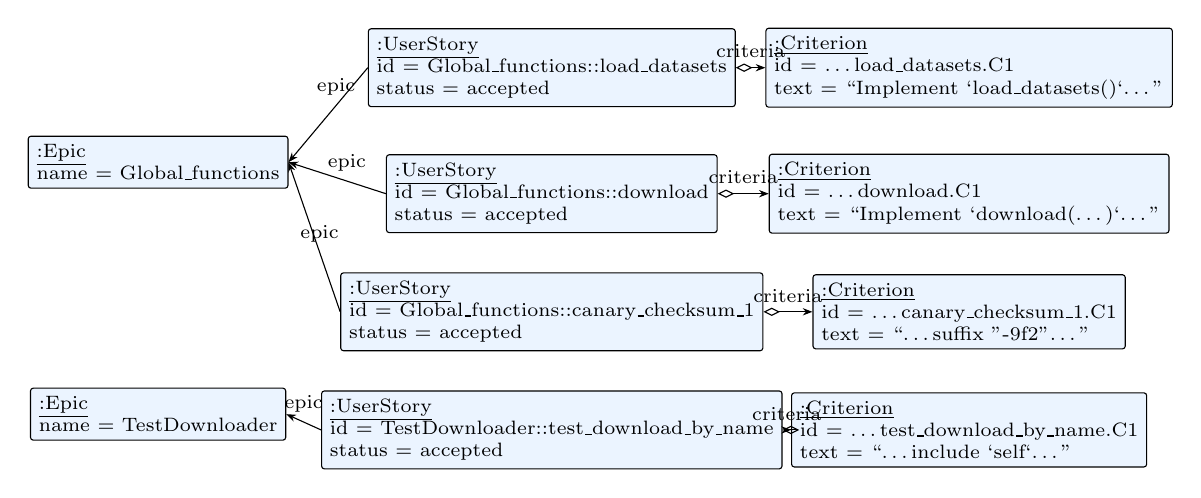
\begin{tikzpicture}[font=\scriptsize, >={Stealth[length=3.5pt]},
  obj/.style={draw, fill=modelbg, align=left, inner sep=3pt, rounded corners=1pt}]
  \node[obj] (e1) at (0,0) {\underline{:Epic}\\name = Global\_functions};
  \node[obj] (e2) at (0,-3.2) {\underline{:Epic}\\name = TestDownloader};
  \node[obj] (s1) at (5,1.2) {\underline{:UserStory}\\id = Global\_functions::load\_datasets\\status = accepted};
  \node[obj] (s2) at (5,-0.4) {\underline{:UserStory}\\id = Global\_functions::download\\status = accepted};
  \node[obj] (s3) at (5,-1.9) {\underline{:UserStory}\\id = Global\_functions::canary\_checksum\_1\\status = accepted};
  \node[obj] (s4) at (5,-3.4) {\underline{:UserStory}\\id = TestDownloader::test\_download\_by\_name\\status = accepted};
  \node[obj] (c1) at (10.3,1.2) {\underline{:Criterion}\\id = \ldots load\_datasets.C1\\text = ``Implement `load\_datasets()`\ldots''};
  \node[obj] (c2) at (10.3,-0.4) {\underline{:Criterion}\\id = \ldots download.C1\\text = ``Implement `download(\ldots)`\ldots''};
  \node[obj] (c3) at (10.3,-1.9) {\underline{:Criterion}\\id = \ldots canary\_checksum\_1.C1\\text = ``\ldots suffix "-9f2"\ldots''};
  \node[obj] (c4) at (10.3,-3.4) {\underline{:Criterion}\\id = \ldots test\_download\_by\_name.C1\\text = ``\ldots include `self`\ldots''};
  \foreach \s in {s1,s2,s3} \draw[->] (\s.west) -- node[above, pos=0.4] {epic} (e1.east);
  \draw[->] (s4.west) -- node[above] {epic} (e2.east);
  \foreach \s/\c in {s1/c1,s2/c2,s3/c3,s4/c4}
     \draw[{Diamond[open,length=6pt]}->] (\s.east) -- node[above] {criteria} (\c.west);
\end{tikzpicture}
\caption{Part of the seeded $M_{\mathit{req}}$ for \texttt{chakin} (4 of the
9 stories). In total: 2 epics, 9 stories, 9 criteria, all \code{accepted}, plus 2 module-level criteria (not shown).}
\label{fig:mreq}
\end{figure}

% ===========================================================================
\section{Step 2: Describe the team as a model}\label{sec:step2}
% ===========================================================================

\subsection{Raw input: who reads whom}

The second design-time input is the collaboration structure, again informal:

\begin{lstlisting}[style=raw]
The Architect works from the accepted user stories.
The Developer works from the Architect's operations.
The Tester writes one test per acceptance criterion.
Each agent writes only its own artifacts.
\end{lstlisting}

\subsection{What happens: the team becomes data}

The team is the megamodel $\team=(A,V,\mathbf{T},\omega,\varphi)$. For
\texttt{chakin} it is constructed by \code{build_team_for_task}
(\Cref{lst:team}). Each line of \Cref{lst:team} fills one component of the
tuple:

\begin{lstlisting}[language=Python, style=model, caption={Building $\team$ for \texttt{chakin} (\file{devbench_agentm2m_config.py}, abridged).}, label={lst:team}]
team = Team()
team.add_agent("Analyst",   "Req");  team.add_view(req_mm,  req_root)   # seeded, Sec. 5
team.add_agent("Architect", "Arch"); team.add_view(arch_mm, arch_root)  # empty
team.add_agent("Developer", "Code"); team.add_view(code_mm, code_root)  # empty
team.add_agent("Tester",    "Test"); team.add_view(test_mm, test_root)  # empty
team.add_handoff("Req2Arch",  RULES / "Req2Arch.agentm2m",  target_mm="Arch")
team.add_handoff("Arch2Code", RULES / "Arch2Code.agentm2m", target_mm="Code")
team.add_handoff("Req2Test",  RULES / "Req2Test.agentm2m",  target_mm="Test")
\end{lstlisting}

\begin{itemize}[nosep]
\item $A=\{\text{Analyst},\text{Architect},\text{Developer},\text{Tester}\}$.
\item $V=\{\MM_{\mathit{req}},\MM_{\mathit{arch}},\MM_{\mathit{code}},\MM_{\mathit{test}}\}$,
each with a live root object; only $M_{\mathit{req}}$ is non-empty.
\item $\mathbf{T}=\{\code{Req2Arch},\code{Arch2Code},\code{Req2Test}\}$. Each
\code{add_handoff} also creates an \emph{empty trace model}
$\TL$ for that hand-off.
\item $\omega$ (write rights) is filled by \code{add_agent}:
$\omega(\text{Architect})=\{\MM_{\mathit{arch}}\}$, and so on. The engine
uses $\omega$ to route obligations: an obligation on an \cls{Operation} goes
to the owner of $\MM_{\mathit{arch}}$, the Architect.
\item $\varphi$ (acceptance) is not a stored formula; it is evaluated over
all registered hand-offs (\Cref{sec:step7}). Adding a hand-off therefore
strengthens $\varphi$ automatically.
\end{itemize}

Because $\team$ is ordinary data kept alongside the running team, it can be
edited while the team runs (\Cref{sec:hot}). This is the models@run.time
idea~\cite{blair2009runtime}.

\paragraph{Two structural invariants} follow from this construction and are
used repeatedly below. (i) \emph{One producer per target type}: \code{Req2Test}
creates \cls{TestCase}s and nothing else creates them; no target object has two
producers. (ii) \emph{Read up, write own}: every hand-off reads upstream views
and writes only the view of its target owner.

% ===========================================================================
\section{Step 3: Write each hand-off as hybrid rules}\label{sec:step3}
% ===========================================================================

\subsection{Raw input: the rule modules}

\Cref{lst:req2arch} is the real \code{Req2Arch} module of the pilot. The
other two, \code{Arch2Code} and \code{Req2Test}, follow in
\Cref{lst:arch2code,lst:req2test}.

\begin{lstlisting}[language=ATL, style=model, caption={\file{devbench_rules/Req2Arch.agentm2m} ($T_1$).}, label={lst:req2arch}]
module Req2Arch;
create OUT : Arch from IN : Req;
uses 'helpers.py';

rule Epic2Component {
  from e : Req!Epic
  to  c : Arch!Component ( name <- e.name ) }

rule Story2Operation {
  from s : Req!UserStory
           (s.status = #accepted)              -- guard
  to  op : Arch!Operation (
    id        <- s.id,                         -- structural
    name      <- s.id.realName(),              -- structural
    component <- s.epic,                       -- structural, resolved via trace
    spec      <- s.criteria.criteriaText(),    -- structural: carried forward, no LLM
    signature <- @llm('Derive a precise Python signature (parameter list and
                   return type, e.g. name(param1, param2) -> ReturnType) for
                   this operation from its acceptance criteria. Respond with
                   ONLY the signature on one line ...',
                   s.criteria),                -- footprint
    @check signature.parses() ) }
\end{lstlisting}

\begin{lstlisting}[language=ATL, style=model, caption={\file{devbench_rules/Arch2Code.agentm2m}.}, label={lst:arch2code}]
module Arch2Code;  create OUT : Code from IN : Arch;
rule Operation2CodeEdit {
  from op : Arch!Operation
  to  ce : Code!CodeEdit (
    name      <- op.name,
    operation <- op,
    body      <- @llm('Implement this operation as a complete Python function
                   ... that satisfies the specification. Output ONLY the raw
                   def block ...',
                   op.codeContext()),          -- footprint: signature + spec
    @check body.compiles() and body.definesName(op.name)
           and body.loads() ) }
\end{lstlisting}

\begin{lstlisting}[language=ATL, style=model, caption={\file{devbench_rules/Req2Test.agentm2m}.}, label={lst:req2test}]
module Req2Test;  create OUT : Test from IN : Req;
rule Criterion2TestCase {
  from c : Req!Criterion
  to  tc : Test!TestCase (
    name      <- c.text,
    criterion <- c,
    oracle    <- @llm('Write a test oracle for this acceptance criterion. The
                   operation under test is available as a function named
                   implementation (do NOT define or import it). Define
                   def test_oracle(): that calls implementation(...) and asserts
                   the criterion holds with at most 3 assert statements. If the
                   operation is a method, implementation is already bound to an
                   instance: pass only the arguments after self, and never
                   construct the class. Output ONLY the raw Python def block.',
                   c.text),
    @check oracle.failsOnStub() ) }
\end{lstlisting}

\subsection{What happens: splitting each rule into structure and value}

The parser splits every rule $r$ into the four parts of the paper's
Definition~1. For \code{Story2Operation}:

\begin{center}
\small
\begin{tabularx}{\textwidth}{@{}l l X@{}}
\toprule
Part & Content & Who decides \\
\midrule
Source pattern $p_r$ & \code{s : Req!UserStory} & engine \\
Guard $g_r$ & \code{s.status = \#accepted} & engine \\
Target pattern $t_r$ & \code{op : Arch!Operation} & engine: \emph{whether} \code{op} exists \\
$B^{\str}_r$ & \code{id}, \code{name}, \code{component}, \code{spec} & engine: identity, symbol name, which component, the criterion text carried forward \\
$B^{\sem}_r$ & \code{signature} & LLM, from footprint \code{s.criteria}, accepted only if \code{parses()} \\
\bottomrule
\end{tabularx}
\end{center}

For each stochastic binding the engine records three things:

\begin{itemize}[nosep]
\item \textbf{Footprint expression.} \code{s.criteria} for \code{signature};
\code{op.codeContext()} (the signature and \code{op.spec}) for \code{body};
\code{c.text} for \code{oracle}. For a
given match, this expression is evaluated to a concrete value, and that value
is the \emph{only} source data rendered into the prompt.
\item \textbf{Validator.} Every validator first \emph{extracts} the code
from the sample (the first fenced block if there is one; otherwise the raw
text, minus a pair of inline backticks around a one-line answer), so that it
judges content, not wrapping: coder models routinely add a prose preamble,
markdown fences or inline backticks even when told not to. A validator that
rejects returns a \emph{reason} (e.g., ``the code must define a top-level
\code{def download(...)}''), which the engine puts into the resample prompt
(\Cref{sec:tokens}). \code{parses()} then
accepts \code{name(args) -> T} (leniently: an optional leading \code{def},
a \code{Class.} qualifier and a trailing colon are allowed);
\code{compiles()} runs Python's compiler on the body,
\code{definesName(op.name)} requires a top-level \code{def} with the
operation's exact name, and \code{loads()} executes the body's top-level
statements (imports and the \code{def}), so an import of a non-existent name
is caught at this binding rather than breaking the assembled module; \code{failsOnStub()} requires an oracle that calls
\code{implementation(...)} \emph{without defining it}, runs it against a stub
that raises \code{NotImplementedError}, and accepts it only if it fails on
the stub with that error or an \code{AssertionError} (a vacuous oracle, or
one that tests its own inline re-implementation, is rejected). An oracle cut
off by the output-token cap is first shortened by up to three unfinished
trailing lines, so a complete \code{test\_oracle} is not discarded because
its last assert was truncated.
\item \textbf{Owner.} The LLM that answers is the one of the target view's
owner, found through $\omega$: the Architect answers \code{signature}, the
Developer \code{body}, the Tester \code{oracle}.
\end{itemize}

\begin{remark}[Why the footprint matters]
The footprint decides three things at once: what the LLM can see, which
source changes can invalidate the value later, and how many input tokens the
call costs. The first pilot's \code{Arch2Code} gave the Developer \emph{only}
\code{op.signature}. That kept change impact very precise, but any detail of
the criterion that is not encoded in the signature (such as the \code{-9f2}
suffix of \code{canary_checksum_1}) could not reach the Developer. The
current rule adds the criterion text, copied structurally into
\code{op.spec} by \code{Req2Arch}: the Developer now sees what it must
implement, while the footprint still reads nothing outside its own story.
We return to this in \Cref{sec:step4-code}.
\end{remark}

% ===========================================================================
\section{Step 4: Run a hand-off}\label{sec:step4}
% ===========================================================================

The runtime executes Algorithm~1 of the paper, i.e., ATL's two-phase execution
made incremental~\cite{jouault2010incremental}. We run \code{Req2Arch} on the
seeded $M_{\mathit{req}}$ and follow each line.

\subsection{Line 1: compute the match set (read-only)}

For every rule the matcher enumerates all source objects of the pattern
type, evaluates the guard, and gives each surviving match a stable key built
from the element keys of its source objects.

\begin{center}\small
\begin{tabular}{@{}l l l@{}}
\toprule
Rule & Candidates & Matches (keys) \\
\midrule
\code{Epic2Component} & 2 epics & \code{e=Epic\#Global_functions}, \code{e=Epic\#TestDownloader} \\
\code{Story2Operation} & 9 stories, guard \code{accepted} & \code{s=UserStory\#Global_functions::load_datasets}, \ldots\ (9 keys) \\
\bottomrule
\end{tabular}
\end{center}

Nothing is written yet. Because $M_{\mathit{req}}$ is read-only while the
hand-off runs, the match set is fixed before any rule fires.

\subsection{Lines 2--3: create one target and one trace link per new match}

The trace model is empty, so all 11 matches are new. For each one the engine
creates an empty target object, appends it to the target root, and records a
trace link. The run report lists them:

\begin{lstlisting}[style=engine, caption={Engine output: created targets of the first \code{Req2Arch} run.}]
created:
  Epic2Component::c::e=Epic#Global_functions
  Epic2Component::c::e=Epic#TestDownloader
  Story2Operation::op::s=UserStory#Global_functions::load_datasets
  Story2Operation::op::s=UserStory#Global_functions::download
  Story2Operation::op::s=UserStory#Global_functions::search
  Story2Operation::op::s=UserStory#TestDownloader::test_download_by_name
  Story2Operation::op::s=UserStory#Global_functions::canary_checksum_1
  ... (4 more canaries)
\end{lstlisting}

The target key has the form \code{rule::targetVar::matchKey}. This is the
point where P1 (lossy hand-offs) is addressed \emph{structurally}: there is
one \cls{Operation} for every accepted story, whether or not any LLM later
does a good job. An operation cannot be ``forgotten'' in a summary.

\subsection{Line 4: delete links whose match disappeared}

No link exists yet, so nothing is deleted. (\Cref{sec:remove} shows this
line at work.)

\subsection{Line 5: evaluate structural bindings, resolving through the trace}

For the match \code{s=UserStory\#Global_functions::download} the engine
evaluates, deterministically:

\begin{enumerate}[nosep]
\item \code{id <- s.id} $\Rightarrow$ \code{"Global_functions::download"}.
\item \code{name <- s.id.realName()} $\Rightarrow$ helper
\code{realName} splits on the last \code{::} $\Rightarrow$ \code{"download"}.
\item \code{component <- s.epic} $\Rightarrow$ evaluates to the \emph{source}
object \code{Epic\#Global_functions}. The target feature \code{component}
expects an \cls{Arch!Component}, and an \cls{Epic} is not one, so the engine
\emph{resolves} it: it looks up the trace link whose source key is
\code{Epic\#Global_functions}, finds target
\code{Epic2Component::c::e=Epic\#Global_functions}, and assigns that
\cls{Component}.
\end{enumerate}

This resolution step is why \code{Epic2Component} exists: without it,
\code{s.epic} would have nothing in $M_{\mathit{arch}}$ to resolve to. Note
also that no LLM has been called so far.

\subsection{Lines 6--13: stochastic bindings, gated by version stamps}

For each match, for each stochastic binding, the engine:

\begin{enumerate}[nosep, label=(\alph*)]
\item evaluates the footprint expression, here \code{s.criteria};
\item computes its digest (SHA-256 of a canonical JSON of the footprint's
primitive attributes, truncated to 16 hex characters);
\item compares it with the stamp stored on the trace link. No stamp yet, so
the binding must be sampled. (Had the binding been escalated earlier on this
very digest, the engine would re-report that escalation and make no call;
\Cref{sec:tokens}.);
\item builds the prompt as \emph{rule prompt} $\oplus$ \emph{rendered
footprint} (nothing else);
\item samples up to $k=2$ times until \code{@check} accepts;
\item on acceptance, writes the value and stores the stamp; after $k$
rejections, records an escalation, stores the digest as a \emph{failed
stamp}, and writes nothing. A transport error (timeout, lost connection) is
not a rejection and stores no failed stamp.
\end{enumerate}

\Cref{lst:prompt-download} is the exact prompt for \code{download}. Note
that the Architect's LLM sees neither the rest of the PRD, nor other stories,
nor any previous conversation.

\begin{lstlisting}[style=llm, caption={Prompt sent for (\code{op download}, \code{signature}).}, label={lst:prompt-download}]
Derive a precise Python signature (parameter list and return type, e.g.
name(param1, param2) -> ReturnType) for this operation from its acceptance
criteria. Respond with ONLY the signature on one line, no markdown code
fences, no explanation.

Context (footprint only):
- Criterion({'id': 'Global_functions::download.C1', 'text': 'Implement
  `download(number: int, name: string, save_dir: string)` on component
  `Global_functions`. This is a free function (not a class method).'})
\end{lstlisting}

In our run, the first sample is prose and is rejected; the second is
accepted:

\begin{lstlisting}[style=llm, caption={Two samples for (\code{op download}, \code{signature}).}]
sample 1: The download operation takes a number, a name and a directory.
          -> @check signature.parses()  = false   (rejected, not written)
sample 2: download(number: int, name: str, save_dir: str) -> None
          -> @check signature.parses()  = true    (accepted, written, stamped)
\end{lstlisting}

The rejected sample never touches $M_{\mathit{arch}}$: a value is committed
only after its validator passes. \Cref{lst:trace-link} shows the trace link
for \code{load_datasets} after acceptance, as persisted by the engine.

\begin{lstlisting}[style=engine, caption={A persisted trace link of $\TL_{\code{Req2Arch}}$, with its stamp.}, label={lst:trace-link}]
{ "rule": "Story2Operation",
  "match_key":  "s=UserStory#Global_functions::load_datasets",
  "source_keys": { "s": "UserStory#Global_functions::load_datasets" },
  "target_key": "Story2Operation::op::s=UserStory#Global_functions::load_datasets",
  "stamps":     { "signature": "79066a260a457952" },
  "footprints": { "signature": [ { "_type": "Criterion",
      "id": "Global_functions::load_datasets.C1",
      "text": "Implement `load_datasets()` on component `Global_functions`. ..." } ] } }
\end{lstlisting}

After \code{Req2Arch}, $M_{\mathit{arch}}$ contains 2 components and 9
operations. The signatures \texttt{qwen3-coder:30b} produced in the logged
run were:

\begin{lstlisting}[style=llm]
load_datasets() -> dict
download(number: int, name: str, save_dir: str) -> None
search(lang: str) -> Any
test_download_by_name(self, name) -> bool
canary_checksum_1(payload: str) -> str
canary_threshold_2(value: int) -> bool
canary_format_3(name: str, count: int) -> str
canary_merge_4(a: list, b: list) -> list
canary_flag_5(text: str) -> str
\end{lstlisting}

\subsection{The next hand-off: \code{Arch2Code}}\label{sec:step4-code}

\code{Arch2Code} runs exactly the same algorithm, now with
$M_{\mathit{arch}}$ as its read-only source. Its 9 matches create 9
\cls{CodeEdit}s; \code{operation <- op} needs no resolution because
\code{op} already has the declared type. The \code{body} prompt for
\code{canary_checksum_1} is:

\begin{lstlisting}[style=llm, caption={Prompt for (\code{ce canary_checksum_1}, \code{body}): signature plus the carried-forward criterion.}]
Implement this operation as a complete Python function or method (a full
"def name(...):" block matching this exact signature) that satisfies the
specification. If you need a library, import it inside the function body.
Output ONLY the raw def block: ...

Context (footprint only):
Signature: canary_checksum_1(payload: str) -> str
Specification:
[Canary] Implement `canary_checksum_1(payload: str) -> str`: it must return
the input string reversed, with the literal suffix "-9f2" appended ...
\end{lstlisting}

This is where the footprint trade-off becomes visible. The Architect's
signature for \code{canary_checksum_1} is \code{canary_checksum_1(payload:
str) -> str}: correct, but the \code{-9f2} rule is not in it. In the
\emph{pre-fix} pilot the \code{body} footprint was the signature alone, so the
Developer could not see the criterion, and the logged \texttt{qwen3-coder:30b}
body computed something plausible but wrong:

\begin{lstlisting}[style=llm, caption={Pre-fix logged body for \code{canary_checksum_1} (qwen3-coder:30b, signature-only footprint).}]
def canary_checksum_1(payload: str) -> str:
    """Calculate a simple checksum for the given payload string."""
    checksum = 0
    for char in payload:
        checksum += ord(char)
    return hex(checksum % 256)[2:].zfill(2)
\end{lstlisting}

The \emph{structure} survived (the operation and its code edit exist, with
the right name and signature). The \emph{content} of the criterion did not,
because that rule did not put it in the Developer's footprint; 0 of 5
canaries survived. The paper's design avoids this by making $T_2$
multi-source (\Cref{sec:multisrc}). The prototype reaches the same
information with a single-source rule: \code{Req2Arch} copies the criterion
text into \code{op.spec} by a \emph{structural} binding, which costs no LLM
call, and the \code{body} footprint reads \code{op.signature} and
\code{op.spec}. With this change, the first re-run
(\texttt{geotext}, \texttt{qwen2.5-coder:7b}) kept \textbf{5 of 5} canaries
through Req$\to$Arch$\to$Code; both baselines kept 0 of 5 on the same run.

\subsection{The third hand-off: \code{Req2Test}, and an escalation}

\code{Req2Test} matches the 9 criteria and creates 9 \cls{TestCase}s; the
\code{oracle} footprint is the criterion text. In the \emph{pre-fix} logs,
every oracle sample was rejected by \code{failsOnStub()} in every run we
inspected. Coder models answer this prompt with a prose preamble plus a fenced
code block (about 400--500 output tokens), and the old validator handed that
raw text to Python's parser, so it never compiled. (In the \texttt{chakin}
\texttt{qwen3-coder:30b} run the model returned empty output, which fails for
the same structural reason.) After $k=2$ samples per test case the engine
recorded escalations instead of writing anything:

\begin{lstlisting}[style=engine, caption={Engine output: escalations of the pre-fix logged run (1 of 9 shown).}]
{ "target_key": "Criterion2TestCase::tc::c=Criterion#Global_functions::load_datasets.C1",
  "binding": "oracle", "rule": "Criterion2TestCase",
  "reason": "@check rejected the sampled value" }
\end{lstlisting}

The test case object \emph{exists} (a criterion cannot be silently dropped),
but its \code{oracle} is empty and it carries no stamp. An escalation is a
visible, addressed failure (it names the target, the binding and the rule),
not a silent one. With the validator now extracting the code block before
judging it, and the prompt stating that \code{implementation} is provided,
8 of 9 oracles were accepted on the first sample in the \texttt{geotext}
re-run; one escalated.

\subsection{Second pass: the fixpoint}

The runtime repeats the hand-offs until a pass changes nothing (at most two
passes in the pilot). In the second pass every match is already covered and
every accepted value has a fresh stamp, so:

\begin{lstlisting}[style=engine]
PASS 2   Req2Arch : +0 created, -0 deleted, 0 resampled
         Arch2Code: +0 created, -0 deleted, 0 resampled
         Req2Test : +0 created, -0 deleted, 0 resampled
\end{lstlisting}

That is, \textbf{zero LLM calls}: accepted bindings have fresh stamps, and
escalated bindings have a failed stamp equal to their current digest, so they
are re-reported without being re-sampled. $\varphi$ stays false while any
escalation is open.

\begin{remark}[What the pre-fix engine did here]
The pre-fix engine stored no stamp for an escalated binding, so pass 2
re-sampled it in full on an unchanged footprint. With all 9 oracles
rejected, the pre-fix call count was $10$ signature samples $+\;9$ bodies
$+\;18$ oracle samples in pass 1 $+\;18$ \emph{identical} retries in pass 2
$=55$ calls, 36 of them for oracles that could not be accepted. These
rejected samples alone accounted for roughly 16k of the run's 18.6k output
tokens on \texttt{geotext}. \Cref{sec:tokens} lists the fixes and their
effect.
\end{remark}

% ===========================================================================
\section{Controlling token usage: when the engine calls an LLM}\label{sec:tokens}
% ===========================================================================

The premise of \tool{} is that the LLM fills in only the values a
deterministic engine cannot compute. That premise is only as good as the
engine's discipline about \emph{when} it asks, \emph{what} it sends, and
\emph{how many tries} it takes to get an acceptable value. The first pilot
had none of that discipline, and \tool{} cost several times more than
free-text hand-offs. This section explains where the tokens went, what we
changed, and why the result can undercut free text.

\subsection{The token cost equation}

A free-text team pays for a few long calls: every role re-reads the whole
upstream transcript, and the cost is roughly fixed per task. \tool{} pays per
stochastic binding instance. For a run, its token cost is
\[
C_{\tool{}} \;=\; \sum_{(t,b)\,\in\,S}\ \sum_{i=1}^{n_{t,b}}
\Big(\underbrace{P}_{\text{preamble}} + \underbrace{|\pi_b|}_{\text{prompt}}
+ \underbrace{|\fp_b(m)|}_{\text{footprint}} + \underbrace{|v_i|}_{\text{output}}
+ \underbrace{|f_{i-1}|}_{\text{feedback}}\Big),
\]
where $S$ is the set of bindings that must be sampled, $n_{t,b}\le k$ is the
number of samples binding $(t,b)$ needs, and $f_{i-1}$ is the feedback
carried into a resample ($f_0=\emptyset$). Every factor has a lever, and the
first pilot left each of them unmanaged:

\begin{center}\small
\begin{tabularx}{\textwidth}{@{}l X X@{}}
\toprule
Factor & What went wrong in the pilot & Lever in \tool{} \\
\midrule
$|S|$: which bindings are sampled & Escalated bindings were re-sampled on every pass with an unchanged footprint (36 of 54 calls on \texttt{geotext}). & Version stamps and \emph{failed stamps}: sample only when the footprint changed since the last acceptance \emph{and} the last escalation. Everything derivable is a structural binding and costs nothing. \\
$n_{t,b}$: samples per binding & Correct values were rejected for their wrapping (prose, fences, inline backticks, a \code{Class.} prefix); rejected samples were retried with the identical prompt and came back identical. & \emph{Extract, then validate}: validators judge content, not wrapping. \emph{Reasoned resampling}: a validator returns why it rejected, and the resample prompt carries the rejected answer and that reason. \\
$|v_i|$: output per sample & Oracles grew assert by assert until the 800-token cap cut them mid-line, which made them unparsable, so they were rejected and re-run. & \emph{Bounded outputs}: the prompt fixes the answer's size (at most 3 asserts); an answer truncated at the cap is recovered by dropping its unfinished tail. \\
$|\fp_b(m)|$: footprint & Each operation's criterion repeated the module-wide acceptance bullets, which made up 65--86\% of every footprint (274 tokens per footprint on \texttt{stocktrends}). & \emph{Minimal footprints}: module-level criteria are held once, as \cls{ModuleCriterion} elements that no per-operation footprint reads (37 tokens per footprint on \texttt{stocktrends}). \\
$P$: preamble & A model's default system prompt was prepended to every call (1.2k tokens for \texttt{devstral:24b}). & \emph{Minimal preamble}: one short system line, identical for every configuration. \\
\bottomrule
\end{tabularx}
\end{center}

\noindent The contrast with free text follows from the equation. Free text
pays for \emph{repetition across roles}: the analyst's summary, the
architect's design and the developer's code are each re-read in full by the
next role. \tool{} pays for \emph{repetition across bindings}: the prompt
text and the preamble recur in every call. With the levers above, each
binding's call is small, about 170 input and 40 output tokens here. So
\tool{} is cheaper to build than free text when a module has few bindings,
and more expensive when it has many. For a change, it is always much
cheaper, because $S$ shrinks to the change's obligations.

\subsection{The calling rule and its bound}

\begin{quote}
A stochastic binding $(t,b)$ is sampled if and only if its footprint digest
differs from both its stamp (last accepted value) and its failed stamp (last
escalation). It is sampled at most $k$ times. Only a sample that fails its
validator counts against $k$, and each resample carries the rejected answer
and the validator's reason.
\end{quote}

\noindent Every other step (matching, creating and deleting targets,
resolving references, copying text forward, deciding impact, deciding
termination) is deterministic and costs no tokens.

\paragraph{The resulting bound.} A run to fixpoint makes at most
$k\cdot|S|$ LLM calls; later passes add calls only for bindings whose
footprint was changed by a value accepted earlier in the same run. For the
first build, $S$ is every binding instance (on \texttt{geotext}: 9
signatures, 9 bodies, 9 oracles, so at most 54 calls with $k=2$, and 27 if
every first sample is accepted; the final run made 28). For a change
$\Delta$, $S$ is exactly $\Obl(\Delta)$ (\Cref{sec:step6}), so \emph{the
cost of a change grows with its obligations, not with the size of the
team's models}. Free-text and shared-schema teams have no such set, so their
honest cost of a change is running their pipeline again.

\paragraph{Validators that protect the whole module.} Two more validators
serve accuracy, but they also stop one bad value from wasting everyone
else's tokens. \code{definesName(op.name)} rejects a body whose \code{def}
has the wrong name. \code{loads()} executes a body's top-level statements
and rejects, e.g., \code{from typing import Context}. Before these checks, a
single such body made the whole assembled module fail to import, which
discarded every other body and all five canaries (\texttt{lice}: 0/5).

\paragraph{What we measure, and how.} Token counts are the provider's own
(Ollama's \code{prompt\_eval\_count}/\code{eval\_count}, OpenAI/Anthropic
\code{usage}), with a length/4 estimate only where a provider reports
nothing. The MAST judge that annotates transcripts is evaluation overhead,
not part of any configuration, and is metered separately
(\code{eval\_tokens}). For RQ2 we report three numbers: \tool{}'s one-off
\emph{build} cost, each configuration's \emph{identification} cost (deciding
what a change affects; zero for \tool{}, which reads it off the run report)
and its \emph{propagation} cost (bringing every artifact up to date; for the
baselines, re-running their pipeline on the changed requirements).

\paragraph{Per-call overhead matters for a many-call design.} \tool{} makes
many short calls where the baselines make a few long ones, so any fixed cost
per call weighs on it disproportionately. The first post-fix run with
\texttt{devstral:24b} showed this: its Ollama model ships a 5.6k-character
agent system prompt (about 1.2k tokens) that Ollama prepends to every call,
which accounted for about 34k of the 38k input tokens of \tool{}'s 28 calls on
\texttt{geotext}, against about 5k for the 4 free-text calls. The prompt is
also the wrong instruction for filling in one value. The Ollama backend now
sends a one-line system prompt for every configuration alike, which reduced
a probe call's input from 1{,}227 to 38 tokens.

\subsection{Results}

\begin{table}[h]
\centering\small
\caption{Build cost (RQ1) with \texttt{qwen2.5-coder:7b} on two example
repositories. \emph{Pre-fix}: archived log, length/4 estimate, MAST judge
included, 800-token output cap. \emph{Final}: all levers of this section,
exact counts, MAST judge excluded, 4096-token output cap for every
configuration. Canaries: the five criterion constants that reached the code.
All 8 repositories and both models are in \Cref{sec:experiments}.}
\label{tab:tokens}
\begin{tabular}{@{}l l r r r r c@{}}
\toprule
& & \multicolumn{2}{c}{Pre-fix} & \multicolumn{2}{c}{Final} & Canaries \\
\cmidrule(lr){3-4}\cmidrule(lr){5-6}
Repository & Configuration & calls & tokens & calls & tokens & (final) \\
\midrule
\multirow{3}{*}{\texttt{geotext}} & \tool{} & 55 & 26.6k & 28 & \textbf{5.8k} & 5/5 \\
 & free text & 5 & 13.8k & 4 & 6.3k & 0/5 \\
 & shared schema & 4 & 5.5k & 3 & 2.8k & 0/5 \\
\midrule
\multirow{3}{*}{\texttt{readtime}} & \tool{} & 99 & 53.5k & 57 & 13.1k & 5/5 \\
 & free text & 5 & 15.9k & 4 & 6.4k & 0/5 \\
 & shared schema & 4 & 9.7k & 3 & 4.2k & 0/5 \\
\bottomrule
\end{tabular}
\end{table}

\noindent On \texttt{geotext} the levers took \tool{}'s build cost from 26.6k
to 5.8k tokens (intermediate stages: 8.3k after the first round of fixes,
8.6k before bounded outputs, with output tokens falling from 18.6k to 3.1k
and then to 1.1k). That is \textbf{below free text (6.3k)}, and \tool{} is
the only configuration whose code kept all five canaries. On
\texttt{readtime}, whose 16 operations give 48 bindings, the build still
costs about $2\times$ free text (13.1k vs.\ 6.4k), down from $3.4\times$
(53.5k vs.\ 15.9k). This is the crossover the cost equation predicts, and
shared schema, with 3 calls and no executable oracles, remains the cheapest
build. \Cref{fig:build,fig:buildsize} show the same pattern on all 8
repositories and both models.

\begin{table}[h]
\centering\small
\caption{Cost of one change (RQ2), \texttt{qwen2.5-coder:7b}, mean over the
24 changes (8 repositories $\times$ tighten, add, remove). Identification:
deciding what the change affects; propagation: bringing every artifact up to
date. Final runs; both models are in \Cref{tab:final}.}
\label{tab:rq2tokens}
\begin{tabular}{@{}l r r r@{}}
\toprule
Configuration & identification & propagation & per change \\
\midrule
\tool{} & 0 & 0.45k & \textbf{0.45k} \\
free text & 0.15k & 8.43k & 8.57k \\
shared schema & 0 & 4.10k & 4.10k \\
\bottomrule
\end{tabular}
\end{table}

\noindent A change costs \tool{} 0.45k tokens on average (0.88k to tighten:
signature, body and oracle of one operation; 0.48k to add; 0 to remove,
which is purely structural). That is about $19\times$ less than free text
and $9\times$ less than shared schema, at precision and recall 1.00. With
\texttt{qwen3.8:27b} the gap is wider (0.42k vs.\ 15.85k and 7.10k). The
pre-fix RQ2 figures (37.4k for \tool{} vs.\ 0.10k for free text) are not
comparable: they metered a full rebuild for \tool{} and only an impact
\emph{question} for free text. \Cref{fig:cumulative} shows when the cheaper
changes repay \tool{}'s build cost.

% ===========================================================================
\section{Step 5: Turn free text into models (\textsc{Lift})}\label{sec:step5}
% ===========================================================================

Agents still reason in text. \textsc{Lift} is the only way new text enters a
model. In the pilot, \texttt{chakin}'s $M_{\mathit{req}}$ is seeded by the
deterministic loader (\Cref{sec:seed}), so \textsc{Lift} is not on the pilot's
path; the engine implements it as a stochastic binding named \code{self}
whose JSON output is parsed into a whole element. The example below is
\emph{illustrative}: it shows what \textsc{Lift} would do for a new
\texttt{chakin} requirement.

\what{Raw input.} The Analyst (or the user) writes:

\begin{lstlisting}[style=raw]
Users should also be able to list all supported languages.
\end{lstlisting}

\what{L1: render as elements of the author's own view.} The Analyst's LLM is
asked to express this as elements of $\MM_{\mathit{req}}$ and returns JSON:

\begin{lstlisting}[style=llm]
{"id": "Global_functions::list_languages", "status": "accepted",
 "criteria": [{"id": "Global_functions::list_languages.C1",
               "text": "Implement `list_languages()`: return the sorted list of
                        distinct values of the Language column of datasets.csv."}]}
\end{lstlisting}

\what{L2: check conformance of $M_{\mathit{req}}\oplus\Delta$.} Every key
must name a declared feature of \cls{UserStory}; required features must be
present; OCL constraints must hold. Here the mandatory reference \code{epic}
is missing, so the candidate is \emph{rejected} and resampled. A second sample
that adds \code{"epic": "Global_functions"} conforms and is applied. A sample
with an unknown field, e.g.\ \code{"priority": "high"}, would also be
rejected (\code{unknown fields for UserStory: ['priority']}, the prototype's
actual message). Note that the prototype's \textsc{Lift}
(\file{engine/lift.py}) currently checks field names and sets primitive
attributes; the checks on the \code{epic} reference and on the nested
criteria follow the paper's design and are not yet implemented there.

\what{L3: apply $\Delta$ and schedule readers.} The new story and criterion
are added to $M_{\mathit{req}}$. Every hand-off that reads $M_{\mathit{req}}$
(\code{Req2Arch}, \code{Req2Test}) is scheduled; from there on, it is exactly
the ``add'' change of \Cref{sec:add}.

\what{What \textsc{Lift} may not do.} \textsc{Lift} writes only into the
author's own view (by $\omega$) and only creates \emph{source} structure for
downstream hand-offs. The Architect may lift an extra \cls{Component} (e.g.,
a \code{DatasetStore}) into $M_{\mathit{arch}}$, but it cannot create or
delete an \cls{Operation} produced by \code{Req2Arch}: hand-off targets are
engine-owned. Hence the targets, references and trace links of each hand-off
remain a function of its source models alone.

% ===========================================================================
\section{Step 6: Handle change with trace models and obligations}\label{sec:step6}
% ===========================================================================

RQ2 injects three PRD changes into \texttt{chakin} after the team has reached
its first fixpoint: tighten a criterion, add an operation, remove an
operation. For each change we show the raw request, the model edit
$\Delta$, how the engine derives the obligations, which LLM calls happen, and
what the baselines did.

The general rule (paper, Step~6) is:
\[
\Obl(\Delta)=\{(t,b)\mid (m,t,r)\in\TL,\ b\in B^{\sem}_r,\ \fp_b(m)\cap\mathit{foot}(\Delta)\neq\emptyset\}.
\]
Operationally, the engine does not diff anything: it re-runs the hand-offs,
recomputes each footprint's digest, and every binding whose digest differs
from its stored stamp \emph{is} an obligation. The obligation is addressed to
the owner of the target view.

\subsection{Change 1: tighten a criterion}\label{sec:tighten}

\what{Raw input.}
\begin{lstlisting}[style=raw]
Tighten the acceptance criterion for `load_datasets`: it must now also raise
ValueError on empty or None input.
\end{lstlisting}

\what{$\Delta$ on $M_{\mathit{req}}$.} The Analyst's criterion text is
edited in place:

\begin{lstlisting}[style=model]
Criterion Global_functions::load_datasets.C1
  text := text + " STRICT UPDATE: must also raise ValueError on empty/None input."
\end{lstlisting}

$\mathit{foot}(\Delta)=\{(\text{\code{load_datasets.C1}},\ \code{text})\}$.

\what{6.1: re-run \code{Req2Arch}, structure first.} The match set is
unchanged (the story is still accepted), so nothing is created or deleted.
Structural bindings produce the same values, except \code{op.spec} of
\code{load_datasets}, which now carries the edited criterion text (a
deterministic copy, no LLM call).

\what{6.2: stamp check on every stochastic binding.}

\begin{center}\small
\begin{tabular}{@{}l l l l@{}}
\toprule
Target & Binding & Footprint & Stamp stored $\rightarrow$ recomputed \\
\midrule
\code{op load_datasets} & \code{signature} & \code{load_datasets.C1} & \code{79066a26...} $\rightarrow$ \code{c79c2b18...} \textbf{stale} \\
\code{op download} & \code{signature} & \code{download.C1} & unchanged \\
\ldots\ (7 more operations) & \code{signature} & their own criterion & unchanged \\
\bottomrule
\end{tabular}
\end{center}

Only one footprint contains the edited criterion, so only one binding is
stale. The Architect is asked for a new signature of \code{load_datasets}
(one LLM call).

\what{6.3: \code{Arch2Code} is obligated directly.} The \code{body}
footprint is \code{op.codeContext()}, which reads \code{op.spec}; the spec
changed in 6.1, so \code{body}'s stamp is stale whatever the Architect
answered, and the Developer re-implements \code{load_datasets} (one call).
This is what the change requires: a \code{ValueError} rule need not alter
the signature, but it must alter the code. Hand-offs whose footprint is the
signature alone behave differently depending on the Architect's answer:

\begin{itemize}
\item \textbf{Case A, same signature.} The model answers
\code{load_datasets() -> dict} again. The value is re-accepted with the new
stamp, but the signature is \emph{unchanged}, so a reader of
\code{op.signature} only, such as the Security Reviewer's \code{Arch2Sec}
(\Cref{sec:hot}), finds a fresh stamp and makes no call.
\item \textbf{Case B, different signature.} The model answers
\code{load_datasets() -> pandas.DataFrame}. Now \code{Arch2Sec}'s stamps are
stale as well and the reviewer re-reviews the operation.
\end{itemize}

\what{6.4: \code{Req2Test}, in parallel.} The \code{oracle} footprint of
\code{tc load_datasets.C1} is \code{c.text}, which changed, so the Tester
gets an obligation too (\code{8e403f24...} $\rightarrow$ \code{13f5b7b9...}).
The Tester's footprint does not go through the Architect, so this obligation
arises whether or not the signature changed.

\begin{lstlisting}[style=engine, caption={Engine output for the tighten change (3 LLM calls).}]
Req2Arch : resampled (Story2Operation::op::s=UserStory#Global_functions::load_datasets, signature)
Arch2Code: resampled (Operation2CodeEdit::ce::op=Operation#Global_functions::load_datasets, body)
Req2Test : resampled (Criterion2TestCase::tc::c=Criterion#Global_functions::load_datasets.C1, oracle)
predicted impact = {load_datasets}      oracle impact = {load_datasets}
\end{lstlisting}

\begin{remark}[Design versus pilot]
In the paper's design, $T_2$'s \code{body} reads the story's criteria through
a second source view, so the code edit is obligated \emph{directly} by the
criterion change (``a 409 need not alter the signature''). The prototype now
has the same obligation through \code{op.spec}. The pre-fix pilot, with a
signature-only footprint, obligated the Developer only in Case B, and so left
stale code whenever the signature survived a behavioral change. Both are sound
with respect to their declared footprints; they differ in what they declare.
This is the ``footprint-bounded vs.\ full-context'' trade-off listed as
future work.
\end{remark}

\subsection{Change 2: add an operation}\label{sec:add}

\what{Raw input.}
\begin{lstlisting}[style=raw]
Add a new operation `extra_feature_op()` to the module: it must return the
literal string 'ADDED_OK'.
\end{lstlisting}

\what{$\Delta$.} A new accepted \cls{UserStory}
\code{Global_functions::extra_feature_op} with one \cls{Criterion} is added
to $M_{\mathit{req}}$.

\what{What happens.} This time the change is in the \emph{match set}, not in
a footprint:
\begin{enumerate}[nosep]
\item \code{Req2Arch}, line~1: a 10th match
\code{s=UserStory\#Global_functions::extra_feature_op}; lines 2--3: a new
\cls{Operation} and trace link; its \code{signature} has no stamp, so it is
sampled (1 call). No existing stamp is affected.
\item \code{Arch2Code}: the new operation is a new match; a new
\cls{CodeEdit} is created and its \code{body} sampled (1 call).
\item \code{Req2Test}: the new criterion is a new match; a new
\cls{TestCase} is created and its \code{oracle} sampled (1 call).
\end{enumerate}
Total: 3 LLM calls. The 9 existing operations are not touched.

\subsection{Change 3: remove an operation}\label{sec:remove}

\what{Raw input.}
\begin{lstlisting}[style=raw]
Remove the operation `test_download_by_name` from the module; it is no longer required.
\end{lstlisting}

\what{$\Delta$.} The story's status is changed: \code{status := "removed"}.

\what{What happens.}
\begin{enumerate}[nosep]
\item \code{Req2Arch}, line~1: the guard \code{s.status = \#accepted} now
fails, so the match disappears. Line~4: its trace link and its target
\cls{Operation} are deleted.
\item \code{Arch2Code}, line~1: the deleted operation is no longer in
$M_{\mathit{arch}}$, so the match disappears; line~4 deletes the
\cls{CodeEdit}. The deletion cascades hop by hop.
\item \code{Req2Test}: the pilot rule has \emph{no} status guard, so the
criterion still matches and its \cls{TestCase} remains (9 test cases,
8 operations). In the paper's design, \code{Criterion2TestCase} carries the
guard and the test case would be deleted as well.
\end{enumerate}
Total: 0 LLM calls; deletion is purely structural.

\begin{lstlisting}[style=engine, caption={Engine output for the remove change.}]
Req2Arch : deleted Story2Operation::op::s=UserStory#TestDownloader::test_download_by_name
Arch2Code: deleted Operation2CodeEdit::ce::op=Operation#TestDownloader::test_download_by_name
Req2Test : (no change)
predicted impact = {test_download_by_name}   oracle impact = {test_download_by_name}
\end{lstlisting}

\subsection{Result on \texttt{chakin}, and why it is exact}

\begin{table}[h]
\centering\small
\caption{RQ2 on \texttt{chakin}, \texttt{qwen3-coder:30b} (pre-fix log; the predicted sets follow from the rules and are unchanged by the fixes, as the \texttt{geotext} re-run confirms). P = precision, R = recall.}
\label{tab:rq2}
\begin{tabular}{@{}l l c c l@{}}
\toprule
Change & Configuration & P & R & Predicted impact set \\
\midrule
\multirow{3}{*}{tighten} & \tool{} & 1.00 & 1.00 & \code{load_datasets} \\
 & free text & 0.25 & 1.00 & all 4 operations \\
 & shared schema & 0.25 & 1.00 & all 4 operations \\
\midrule
\multirow{3}{*}{add} & \tool{} & 1.00 & 1.00 & \code{extra_feature_op} \\
 & free text & 0.20 & 1.00 & all 4 + \code{extra_feature_op} \\
 & shared schema & 0.20 & 1.00 & all 4 + \code{extra_feature_op} \\
\midrule
\multirow{3}{*}{remove} & \tool{} & 1.00 & 1.00 & \code{test_download_by_name} \\
 & free text & 0.25 & 1.00 & all 4 operations \\
 & shared schema & 0.25 & 1.00 & all 4 operations \\
\bottomrule
\end{tabular}
\end{table}

\tool{}'s predicted set is read off the run report (created, deleted and
re-sampled targets), not asked from an LLM. It is exact because
(i) each story's footprints read only that story's data, (ii) every change
touches only one story, and (iii) the stamp check finds exactly the bindings
whose footprint contains the edited data. This is why the result is the same
for all three models: it follows from the rules, not from generation quality.

\paragraph{Cost of a change.} The same obligations determine the cost: the
engine samples exactly the bindings in $\Obl(\Delta)$ (\Cref{sec:tokens}).
Tighten costs 3 calls (signature, body, oracle of one operation), add costs
3 (the new operation's three bindings), remove costs 0. The baselines cannot
act on an impact set, because their artifacts are one undifferentiated
transcript or implementation blob, so they regenerate. On \texttt{geotext}
(\Cref{tab:tokens}) a change cost \tool{} 0.58k tokens on average, versus
6.94k for free text and 3.00k for shared schema. The pre-fix logs reported
the opposite ordering (34--37k for \tool{} vs.\ under 600 for free text),
because they charged \tool{} for rebuilding the whole team before each change
and charged free text only for asking which operations were affected.

% ===========================================================================
\section{When several hand-offs fire: fan-out, cascades, concurrent changes}\label{sec:multi}
% ===========================================================================

Real teams do not change one thing at a time, and one agent's output is often
read by several others. This section walks through what the engine does in
those situations, using the \texttt{chakin} team \emph{after} the Security
Reviewer has joined (\Cref{sec:hot}), so that four hand-offs are registered:
\code{Req2Arch}, \code{Arch2Code}, \code{Req2Test}, \code{Arch2Sec}.

\subsection{Fan-out: one view read by several hand-offs}

$M_{\mathit{req}}$ is read by \code{Req2Arch} and \code{Req2Test};
$M_{\mathit{arch}}$ is read by \code{Arch2Code} and \code{Arch2Sec}. Each
hand-off has its \emph{own} trace model and its \emph{own} stamps, so the
readers never coordinate with each other:

\begin{itemize}[nosep]
\item Each reader computes its own match set over the same source and creates
elements of \emph{disjoint} types in \emph{different} target views
(\cls{Operation} vs.\ \cls{TestCase}; \cls{CodeEdit} vs.\
\cls{SecurityReview}). No target object has two producers, so there is
nothing to merge and no write conflict.
\item Two readers can depend on the very same data. After the HOT, the trace
links of \code{Arch2Code} (\code{body}) and \code{Arch2Sec} (\code{notes},
\code{risk}) for \code{load_datasets} both digest \code{op.signature}:
\code{Arch2Sec}'s footprint is the signature alone, and \code{Arch2Code}'s
\code{op.codeContext()} contains it. One change to that signature therefore
obligates both the Developer and the Security Reviewer, independently; a
change to \code{op.spec} obligates only the Developer.
\end{itemize}

\subsection{Cascades: obligations travel hop by hop}

A re-accepted value in $M_j$ is itself a change to $M_j$. The engine does not
need a separate message to tell downstream agents; the downstream hand-off's
own stamp check detects it. \Cref{fig:cascade} shows the path of the
tighten change from \Cref{sec:tighten}, Case B.

\begin{figure}[h]
\centering
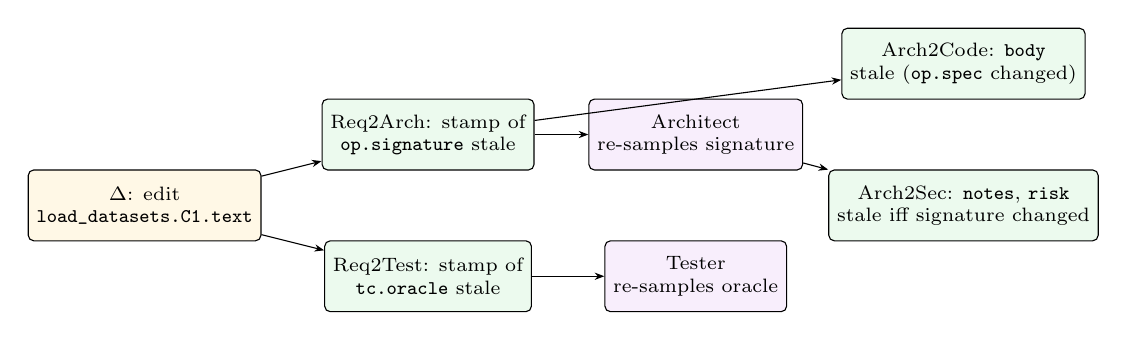
\begin{tikzpicture}[font=\scriptsize, >={Stealth[length=3.5pt]},
  box/.style={draw, rounded corners=2pt, align=center, inner sep=3pt, minimum height=9mm},
  ch/.style={box, fill=rawbg}, st/.style={box, fill=enginebg}, ll/.style={box, fill=llmbg}]
  \node[ch] (d) at (0,0) {$\Delta$: edit\\\code{load_datasets.C1.text}};
  \node[st] (s1) at (3.6,0.9) {Req2Arch: stamp of\\\code{op.signature} stale};
  \node[st] (s2) at (3.6,-0.9) {Req2Test: stamp of\\\code{tc.oracle} stale};
  \node[ll] (l1) at (7.0,0.9) {Architect\\re-samples signature};
  \node[ll] (l2) at (7.0,-0.9) {Tester\\re-samples oracle};
  \node[st] (s3) at (10.4,1.8) {Arch2Code: \code{body}\\stale (\code{op.spec} changed)};
  \node[st] (s4) at (10.4,0.0) {Arch2Sec: \code{notes}, \code{risk}\\stale iff signature changed};
  \draw[->] (d) -- (s1); \draw[->] (d) -- (s2);
  \draw[->] (s1) -- (l1); \draw[->] (s2) -- (l2);
  \draw[->] (s1) -- (s3); \draw[->] (l1) -- (s4);
\end{tikzpicture}
\caption{Hop-by-hop propagation of one criterion edit after the reviewer has
joined. Green: deterministic stamp checks; purple: LLM calls. \code{Req2Arch}
copies the edited text into \code{op.spec}, so \code{Arch2Code} is obligated
directly. If the Architect re-samples an identical signature, the
\code{Arch2Sec} check finds fresh stamps and that path stops there.}
\label{fig:cascade}
\end{figure}

An identical re-sample stops only the paths it alone determines. The
Tester's and the Developer's obligations do not depend on the Architect's
answer, so they are raised regardless.

\subsection{Concurrent changes from different sources}

\what{Raw input.} Two requests arrive before the team runs again:
\begin{lstlisting}[style=raw]
(1) Tighten the acceptance criterion for `load_datasets`: ... raise ValueError ...
(2) Add a new operation `extra_feature_op()` ... return the literal string 'ADDED_OK'.
\end{lstlisting}

Both are applied to $M_{\mathit{req}}$ (one criterion edited, one story
added), and the runtime then iterates over all four hand-offs in
registration order until a pass is quiet. The real engine output:

\begin{lstlisting}[style=engine, caption={Engine output: two concurrent Analyst changes, four hand-offs.}, label={lst:multi}]
PASS 1
 Req2Arch : created  op extra_feature_op
            resampled op load_datasets.signature, op extra_feature_op.signature
 Arch2Code: created  ce extra_feature_op
            resampled ce load_datasets.body, ce extra_feature_op.body
 Req2Test : created  tc extra_feature_op.C1
            resampled tc load_datasets.C1.oracle, tc extra_feature_op.C1.oracle
 Arch2Sec : created  sr extra_feature_op
            resampled sr load_datasets.{notes,risk}, sr extra_feature_op.{notes,risk}
PASS 2
 (all four hand-offs: +0 created, -0 deleted, 0 resampled)      -> fixpoint
LLM calls: 10        phi after the run: true
\end{lstlisting}

Step by step:
\begin{enumerate}[nosep]
\item \textbf{Req2Arch} sees one new match (\code{extra_feature_op}) and one
stale stamp (\code{load_datasets}). 2 calls.
\item \textbf{Arch2Code} runs after \code{Req2Arch} in the same pass, so it
already sees the new operation and the changed signature: one new match, one
stale stamp. 2 calls.
\item \textbf{Req2Test} sees one new criterion and one edited criterion. 2 calls.
\item \textbf{Arch2Sec} sees the same two operations as \code{Arch2Code}; each
review has two stochastic bindings. 4 calls.
\item \textbf{Pass 2} finds every match covered and every stamp fresh:
fixpoint, $\varphi$ holds.
\end{enumerate}

The 8 untouched operations and their 8 code edits, 8 test cases and 8
reviews cost nothing. Three properties make this safe:

\begin{itemize}[nosep]
\item \textbf{Order independence of the changes.} Stamps are digests of the
\emph{current} footprint, not a log of events. Applying (1) then (2), or (2)
then (1), or both at once, leads to the same state and the same obligations.
\item \textbf{Order independence within a hand-off.} Sources are read-only
while a hand-off runs and each target has one producer, as in ATL.
\item \textbf{Order of hand-offs affects cost, not result.} Registration
order follows the data flow here, so one pass suffices. Had \code{Arch2Code}
run before \code{Req2Arch}, it would have found nothing to do in pass 1 and
done its work in pass 2; the final models would be identical.
\end{itemize}

\subsection{Multi-source hand-offs}\label{sec:multisrc}

In the paper, $T_2$ reads two views: the Developer sees the operation
\emph{and} the story's criteria. A hypothetical \texttt{chakin} version of
the rule would be:

\begin{lstlisting}[language=ATL, style=model, caption={Illustrative multi-source \code{Arch2Code} (the paper's design; the prototype uses \code{op.spec} instead).}]
module Arch2Code; create OUT : Code from IN1 : Arch, IN2 : Req;
rule Operation2CodeEdit {
  from op : Arch!Operation, s : Req!UserStory (op.id = s.id)
  to  ce : Code!CodeEdit (
    name <- op.name,  operation <- op,
    body <- @llm('Implement this operation ...',
                 Sequence{op.signature, s.criteria}),
    @check body.compiles() ) }
\end{lstlisting}

Now a match is a \emph{pair} (operation, story), its key is
\code{op=Operation\#...|s=UserStory\#...}, and the footprint spans both views.
Consequences for \texttt{chakin}: the Developer's prompt for
\code{canary_checksum_1} contains the \code{-9f2} rule, and a criterion
edit obligates the code edit directly, even when the signature does not
change. The prototype gets both effects with a single-source rule: the
structural binding \code{spec <- s.criteria.criteriaText()} in
\code{Req2Arch} carries the criterion into $M_{\mathit{arch}}$ at no LLM
cost, and \code{Arch2Code} reads it from there. The cost, in either form, is
a larger prompt (about 100 input tokens per body here), and a coarser impact
set whenever criteria change often.

\subsection{Conflicts, cycles and failures}

\begin{itemize}[nosep]
\item \textbf{Joint constraints across bindings.} Values accepted one by one
may still violate a constraint of the target view as a whole (in the paper:
two signatures disagreeing on \code{TaskId}). Such a violation escalates all
bindings involved rather than picking a winner.
\item \textbf{Cycles.} The \texttt{chakin} network is acyclic, and the
runtime caps the number of passes. In a cyclic network (e.g., a Developer
feeding back into the Architect's view), the paper schedules with the
conservative strategy of Klare and Gleitze~\cite{klare2023termination}, as in
networks of bidirectional transformations~\cite{stevens2020networks}, which is guaranteed to terminate
but may fail; failure is escalated.
\item \textbf{Exhausted budget.} A binding that fails $k$ times is
escalated and left unwritten, and its footprint digest is stored as a failed
stamp. Later passes re-report the escalation without calling the LLM, and it
keeps $\varphi$ false until someone resolves it: by changing the footprint
(e.g., clarifying the criterion), which earns a fresh budget of $k$, or by
editing the rule or validator.
\end{itemize}

% ===========================================================================
\section{Step 7: Know when the team is done}\label{sec:step7}
% ===========================================================================

$\varphi$ is computed by the engine from the models, not claimed by an agent.
For each registered hand-off it checks: (1) every current match is covered by
a trace link; (2) the last run produced no escalation. (The paper's full
$\varphi$ additionally requires fresh stamps and executes oracles for each
\cls{TestRun} of $T_3$, which the pilot does not have.)

\begin{center}\small
\begin{tabular}{@{}l c c c@{}}
\toprule
Check on \texttt{chakin} & scripted run & pre-fix qwen3 run & reason \\
\midrule
All matches covered (3 hand-offs) & \cmark & \cmark & structure is engine-built \\
No escalations & \cmark & \xmark & 9 oracles rejected by \code{failsOnStub()} \\
\midrule
$\varphi$ & \textbf{true} & \textbf{false} & \\
\bottomrule
\end{tabular}
\end{center}

In the pre-fix run, a Tester that announces ``all tests written'' cannot end
the run: the model state says 9 test cases have no accepted oracle
(MAST FM-1.5 and FM-3.1, unaware of termination and premature termination).
Note that $\varphi$ is about the \emph{coordination} being complete, not about
the code being correct: DevBench's own unit and acceptance tests failed for
\texttt{chakin} in every configuration and model, and still fail for
\texttt{geotext} after the fixes, in every configuration.

% ===========================================================================
\section{Adding a new agent at runtime (higher-order transformation)}\label{sec:hot}
% ===========================================================================

\subsection{Raw input: the lead's request}

After the first fixpoint, the team lead asks:
\begin{lstlisting}[style=raw]
Add a Security Reviewer who reviews every API operation for
authentication/authorization concerns and rates its risk (low, medium, high).
\end{lstlisting}

\subsection{What happens, step by step}

\what{H1: turn the request into a relation model.} The request names a new
agent, a new view and the existing element it relates to (\cls{Operation}).
It is captured as a \code{TeamChange}, the relation model a
HOT~\cite{tisi2009hot} consumes; the chain from relation model to
trace-generating transformation follows MeTAGeM-Trace~\cite{vara2014metagem},
applied at runtime.
The Security Reviewer's view metamodel is new, but small:

\begin{lstlisting}[language=Python, style=model, caption={$\MM_{\mathit{sec}}$ (\file{devbench_sec_metamodel.py}, abridged).}]
review = b.eclass("SecurityReview")
b.attribute(review, "notes")
b.attribute(review, "risk")
b.reference(review, "operation", arch_mm.get("Operation"))   # read reference into Arch
\end{lstlisting}

The relation ``each \cls{SecurityReview} is about one \cls{Operation}''
becomes the rule of the new hand-off $T_5$:

\begin{lstlisting}[language=ATL, style=model, caption={\file{devbench_rules/Arch2Sec.agentm2m} ($T_5$).}]
module Arch2Sec;  create OUT : Sec from IN : Arch;
rule Operation2Review {
  from op : Arch!Operation
  to  sr : Sec!SecurityReview (
    operation <- op,
    notes <- @llm('Summarize any authentication/authorization concerns for this
                   operation signature', op.signature),
    risk  <- @llm('Rate the security risk ... exactly one of low, medium, high.',
                   op.signature),
    @check risk.parsesRisk() ) }
\end{lstlisting}

\what{H2: apply the HOT to the team model.} This is the entire glue the
integrator writes (7 non-blank lines, counted by
\file{hot_reviewer_rq3.py}):

\begin{lstlisting}[language=Python, style=model, caption={The 7 lines of glue.}, label={lst:glue}]
sec_mm = build_sec_mm(team.views["Arch"])
sec_root = sec_mm.get("SecModel")()
apply_hot(team, TeamChange(
    agent_name="SecurityReviewer", view=sec_mm, view_root=sec_root,
    handoff_name="Arch2Sec", rule_path=RULES_DIR / "Arch2Sec.agentm2m",
))
runtime.run_to_fixpoint()
\end{lstlisting}

\code{apply_hot} performs three edits on $\team$, one per component of the
tuple it touches:

\begin{lstlisting}[style=engine, caption={$\team$ before and after the HOT (engine state).}]
A      : Analyst, Architect, Developer, Tester   +  SecurityReviewer
V      : Req, Arch, Code, Test                   +  Sec
omega  : SecurityReviewer -> {Sec}               (new entry; others unchanged)
T      : Req2Arch, Arch2Code, Req2Test           +  Arch2Sec
traces : Req2Arch 11 links, Arch2Code 9, Req2Test 9,  Arch2Sec 0  (fresh, empty)
phi    : now also requires Arch2Sec's matches to be covered and escalation-free
\end{lstlisting}

The HOT is applied \emph{between} two iterations of the runtime's outer loop,
never in the middle of a hand-off, so no running transformation sees a
half-changed team.

\what{H3: the new hand-off runs against existing models.} On the next
\code{run_to_fixpoint}, \code{Arch2Sec} computes its match set over the
\emph{existing} $M_{\mathit{arch}}$: 9 operations. Its trace model is
empty, so all 9 matches are new, and the reviewer receives obligations for
every operation that existed before it arrived. Nobody enumerated them by
hand.

\begin{lstlisting}[style=engine, caption={First run after the HOT.}]
Req2Arch : +0 created, 0 resampled         (nothing changed upstream)
Arch2Code: +0 created, 0 resampled
Req2Test : +0 created, 0 resampled
Arch2Sec : +9 created  (one SecurityReview per existing Operation)
           18 resampled (notes + risk for each of the 9)
LLM calls: 18      retroactive coverage: 9/9 = 1.00      phi: true
\end{lstlisting}

\begin{lstlisting}[style=engine, caption={Resulting trace link in $\TL_{\code{Arch2Sec}}$.}]
{ "rule": "Operation2Review",
  "match_key": "op=Operation#Global_functions::download",
  "target_key": "Operation2Review::sr::op=Operation#Global_functions::download",
  "stamps":     { "notes": "8dec46b3fdb87fa5", "risk": "8dec46b3fdb87fa5" },
  "footprints": { "notes": "download(number: int, name: str, save_dir: str) -> None",
                  "risk":  "download(number: int, name: str, save_dir: str) -> None" } }
\end{lstlisting}

\what{H4: from now on, the reviewer is a normal team member.} Every later
change is propagated to the reviewer by the mechanism of
\Cref{sec:step6,sec:multi}, with no additional glue: \Cref{lst:multi} already
shows \code{Arch2Sec} receiving obligations for a tightened and an added
operation.

\subsection{What the baselines need instead}

Free-text and shared-schema (PatchBoard-style~\cite{zhang2026patchboard})
teams have no team model to transform. Adding the
same reviewer means editing each orchestration file by hand: enumerate every
existing operation, build a review prompt per operation, append the turn,
store the output. \file{hot_reviewer_rq3.py} keeps this retrofit as a
literal snippet of 11 non-blank lines, needed once per baseline config file,
i.e., 22 lines, versus 7 for \tool{}. More importantly, the retrofit reviews
the operations that exist \emph{now}; operations added later are reviewed
only if someone remembers to call it again.

% ===========================================================================
\section{The experiments: setup, results and discussion}\label{sec:experiments}
% ===========================================================================

The walkthrough so far used one repository to explain \emph{how} \tool{}
works. This section reports \emph{how well} it works: on 8 repositories,
with two different LLMs, against two other ways of connecting the same four
agents. Every number and figure below is computed from the run logs by
\file{evaluation/analysis/make_two_model_figures.py}, which also writes the
per-repository data to \file{evaluation/results/csv/devbench\_two\_model\_per\_repo.csv}.

\subsection{What we ran}

\paragraph{Three ways to connect the same team.} All three configurations
use the same four roles (Analyst, Architect, Developer, Tester), the same
LLM and the same requirements.
\begin{itemize}[nosep]
\item \textbf{Free text (F).} Each agent writes a free-text message, and the
next agent reads it. This is how most agent frameworks work today.
\item \textbf{Shared schema (S).} All agents write into one shared,
schema-checked document (in the style of PatchBoard). The format is
checked, but nothing records which piece of the design belongs to which
requirement.
\item \textbf{\tool{} (A).} Each hand-off is a hybrid transformation as
described in Steps~1--7: the engine builds the structure, and the LLM only
fills in values (signatures, code bodies, test oracles), one binding at a
time.
\end{itemize}

\paragraph{Eight repositories.} We use the Python repositories of DevBench
whose own reference solution passes their own tests on our machine. That
check matters: if even the reference fails, a failure tells us nothing about
the agents. Two of the ten repositories failed it (TextCNN needs an old
dataset URL, and Hybrid\_Images breaks with the current numpy), so we left
them out. The remaining eight range from 9 to 22 operations, including five
extra ``canary'' operations per repository (below).

\paragraph{Two models, and why only two.} We ran every experiment with
\texttt{qwen2.5-coder:7b} and \texttt{qwen3.8:27b}. They differ in the ways
that could change our results: size (7 vs.\ 27 billion parameters),
training (code-specialized vs.\ general-purpose), generation (Qwen~2.5 vs.\
Qwen~3.8), and how much they write. Two models are enough for this pilot's
question. Several of our claims (exact change impact, coverage after adding
an agent, the cap on LLM calls) are supposed to come from the rules, not
from the model. So what we need to see is whether they stay the same when
the model changes, while the baselines' results should move. Both models
run on one workstation, so anyone can repeat the experiment, and the local
runtime reports exact token counts per call. Both models are from the Qwen
family; checking other families is future work.

\paragraph{What we measured.}
\begin{itemize}[nosep]
\item \textbf{Canaries (fidelity).} We add five made-up requirements to every
repository, each pinned to an arbitrary constant that cannot be guessed, e.g.,
``reverse the string and append \code{-9f2}''. After the team finishes, a test
checks whether each constant made it into the code. A canary that fails was
lost somewhere between the Analyst and the Developer.
\item \textbf{Build tokens.} All LLM tokens (input and output) one
configuration spends to go from the requirements to code and tests, once.
\item \textbf{Change: precision, recall and tokens.} We then make three edits
to each repository's requirements (tighten one criterion, add one operation,
remove one operation). For each edit we check which operations each
configuration says are affected against the truth (exactly the edited
operation), and count the tokens needed to bring everything up to date.
\item \textbf{Adding an agent at runtime.} We add a Security Reviewer mid-run
and count how many existing operations it reviews.
\end{itemize}

\paragraph{Same settings for everyone.} Temperature 0.2, one run per
repository and model, at most 2 samples per binding for \tool{}, an output cap
of 4096 tokens per call, the same one-line system prompt, and the model's
hidden ``thinking'' switched off, for every configuration.

\subsection{All results in one table}

\begin{table}[!htbp]
\centering\small
\caption{Results on 8 DevBench repositories. F = free text, S = shared
schema, A = \tool{}. Tokens in thousands: mean per repository (build) or per
change (24 changes per model). $^\dagger$Includes one module cut off at the
4096-token output cap (F on \texttt{stocktrends}, S on \texttt{lice}).}
\label{tab:final}
\begin{tabular}{@{}l ccc ccc@{}}
\toprule
& \multicolumn{3}{c}{\texttt{qwen2.5-coder:7b}} & \multicolumn{3}{c}{\texttt{qwen3.8:27b}} \\
\cmidrule(lr){2-4}\cmidrule(l){5-7}
Measure & F & S & A & F & S & A \\
\midrule
Canaries reaching the code (of 40) & 7 & 0 & \textbf{40} & 25$^\dagger$ & 5$^\dagger$ & \textbf{40} \\
DevBench acceptance tests passed (of 8) & 0 & 0 & 0 & 0 & 0 & 0 \\
MAST P1\,/\,P2 modes flagged per run & 0\,/\,0 & 0\,/\,0 & 0\,/\,0.12 & 0.12\,/\,0.62 & 0.12\,/\,0.75 & 0\,/\,1.12 \\
Build tokens & 8.3 & \textbf{3.9} & 11.7 & 16.5 & \textbf{6.8} & 12.5 \\
LLM calls to build (range over repos) & 4 & 3 & 28--83 & 4 & 3 & 27--73 \\
\midrule
Change impact: precision & 0.65 & 0.14 & \textbf{1.00} & 0.79 & 0.14 & \textbf{1.00} \\
Change impact: recall & 0.75 & 1.00 & \textbf{1.00} & 0.79 & 1.00 & \textbf{1.00} \\
Tokens per change & 8.57 & 4.10 & \textbf{0.45} & 15.85 & 7.10 & \textbf{0.42} \\
\midrule
Existing operations reviewed after adding an agent & -- & -- & 118/118 & -- & -- & 118/118 \\
Lines of glue code to add that agent & 11 & 11 & \textbf{7} & 11 & 11 & \textbf{7} \\
\bottomrule
\end{tabular}
\end{table}

\noindent\textbf{How to read it.} Each row is one measure, and each column
is one configuration with one model. Bold marks the best value in a row for
each model.

\noindent\textbf{What it shows, in short.} \tool{} wins every measure about
\emph{information} and \emph{change}. Every canary survived, every change
impact was exact, every existing operation was reviewed, and a change cost
19--38 times fewer tokens than with free text. It does \emph{not} win
building from scratch: shared schema is always cheapest, and with the
smaller model free text is cheaper too. No configuration passed DevBench's
own acceptance tests. The following subsections go through each measure with
a figure.

\subsection{Fidelity: do the requirements reach the code?}

\begin{figure}[!htbp]
\centering
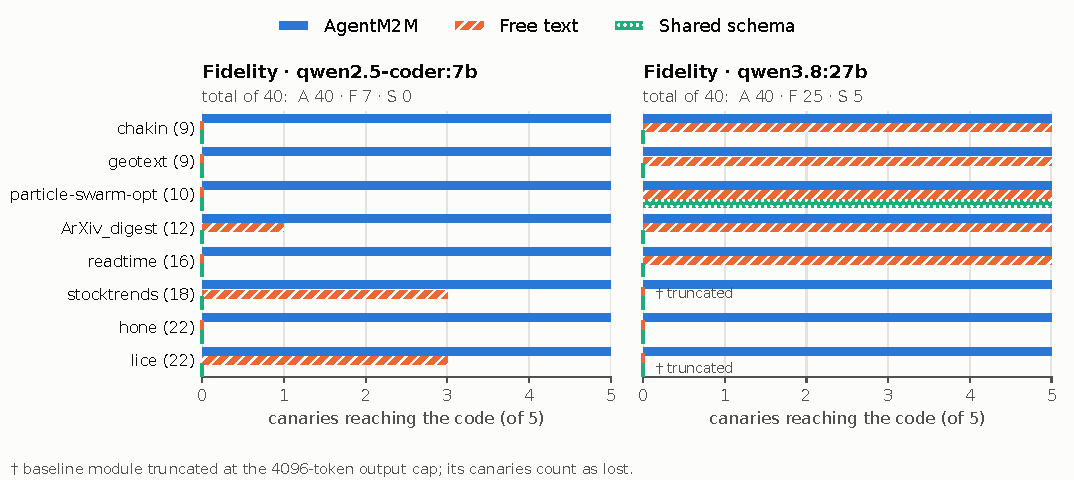
\includegraphics[width=\textwidth]{devbench_two_model_canary.pdf}
\caption{Canaries (of 5) that reached the code, per repository (operation
count in brackets). A short coloured tick at 0 marks a zero.}
\label{fig:canary}
\end{figure}

\noindent\textbf{What we did.} For each repository and configuration we
counted how many of the five canary constants appear, correctly, in the
final code (\Cref{fig:canary}).

\noindent\textbf{How to read it.} One row per repository, one bar per
configuration. A full bar (5) means nothing was lost on the way from the
Analyst to the Developer.

\noindent\textbf{What we see.} \tool{}'s bars are full on every repository,
with both models: 40 of 40. With the small model, free text kept 7 of 40,
and only on three repositories; shared schema kept none. With the large
model, free text did much better (25 of 40) but still lost all five on
\texttt{hone} and \texttt{lice}. On \texttt{stocktrends}, its Developer's
module was cut off at the output cap, marked $\dagger$. Shared schema kept
canaries on one repository only.

\noindent\textbf{Why.} In free text, each agent rewrites what it received in
its own words, and details like ``append \code{-9f2}'' get summarized away. A
bigger model summarizes more carefully, which explains the jump from 7 to 25,
but it still drops things. In \tool{}, the criterion text is copied into the
Architect's model by a structural binding, so no LLM rewrites it, and it is
part of the Developer's footprint. The Developer sees the exact sentence,
whatever the model.

\subsection{Build cost: what does it cost to build once?}

\begin{figure}[!htbp]
\centering
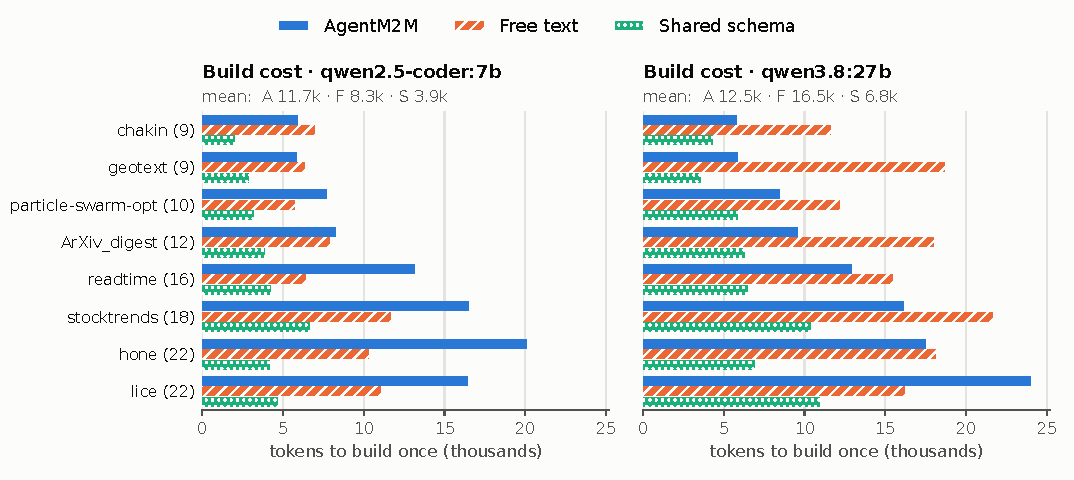
\includegraphics[width=\textwidth]{devbench_two_model_build.pdf}
\caption{Tokens to build the whole module once, per repository.}
\label{fig:build}
\end{figure}

\begin{figure}[!htbp]
\centering
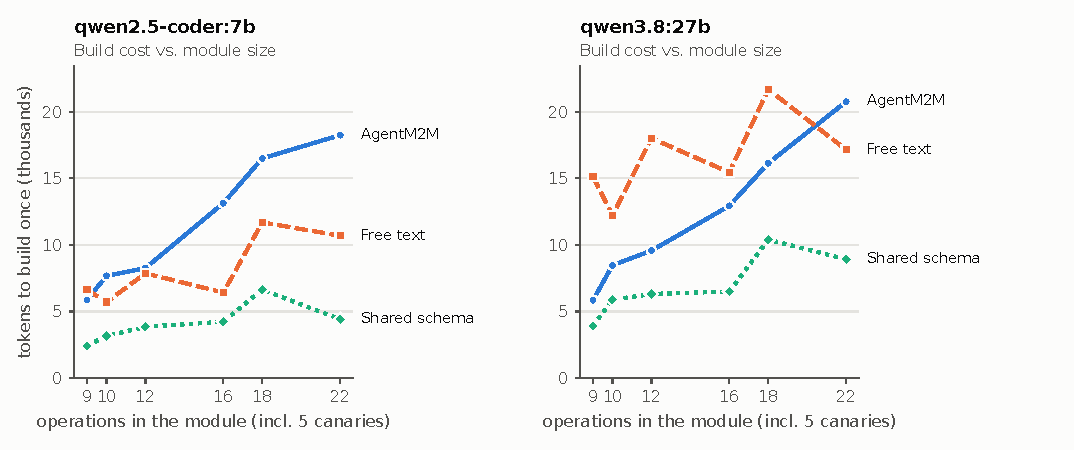
\includegraphics[width=\textwidth]{devbench_two_model_line_build_vs_size.pdf}
\caption{Build tokens against module size (number of operations; repositories
of equal size are averaged).}
\label{fig:buildsize}
\end{figure}

\noindent\textbf{What we did.} We counted all tokens each configuration
spent building the module once (\Cref{fig:build}), and plotted the same
numbers against the number of operations in the module
(\Cref{fig:buildsize}).

\noindent\textbf{How to read it.} Shorter bars and lower lines are cheaper.
Both model panels use the same scale, so they can be compared directly.

\noindent\textbf{What we see.} Shared schema is the cheapest everywhere:
three LLM calls, and no executable test oracles. \tool{}'s cost is almost
the same with both models (for example 5.8k and 5.9k on \texttt{geotext},
11.7k and 12.5k on average), and it grows steadily with the number of
operations, from about 6k at 9 operations to about 20k at 22. Free text's
cost jumps with the model: its average doubles from 8.3k to 16.5k with the
larger model. As a result, \tool{} is cheaper than free text on 2 of 8
repositories with the small model (the two smallest) but on 7 of 8 with the
large model; only on \texttt{lice} is it more expensive (24.0k vs.\ 16.2k).

\noindent\textbf{Why.} \tool{} makes one small call per binding (27--83 calls
per repository), and each call is short because the prompt fixes the
answer's size (\Cref{sec:tokens}). So its cost follows the number of
bindings, not the model's style. Free text makes only four calls, but each
agent writes as much as the model likes and the next agent reads all of it,
so its cost follows how much the model writes. A bigger, chattier model
therefore makes free text more expensive and leaves \tool{} almost
unchanged.

\subsection{Change cost: what does one change cost?}

\begin{figure}[!htbp]
\centering
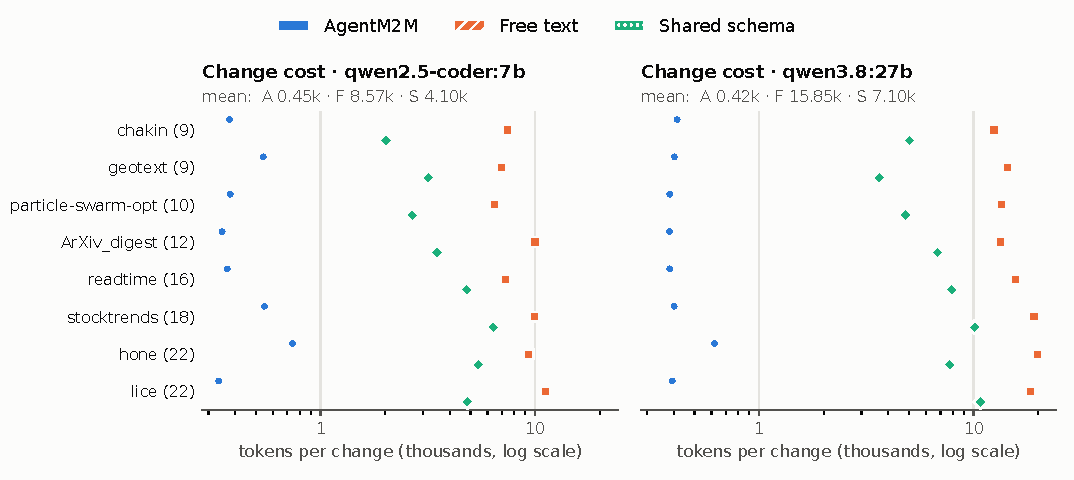
\includegraphics[width=\textwidth]{devbench_two_model_change.pdf}
\caption{Tokens to bring everything up to date after one requirement change,
mean of three changes per repository. Log scale: each grid step is ten
times more.}
\label{fig:change}
\end{figure}

\begin{figure}[!htbp]
\centering
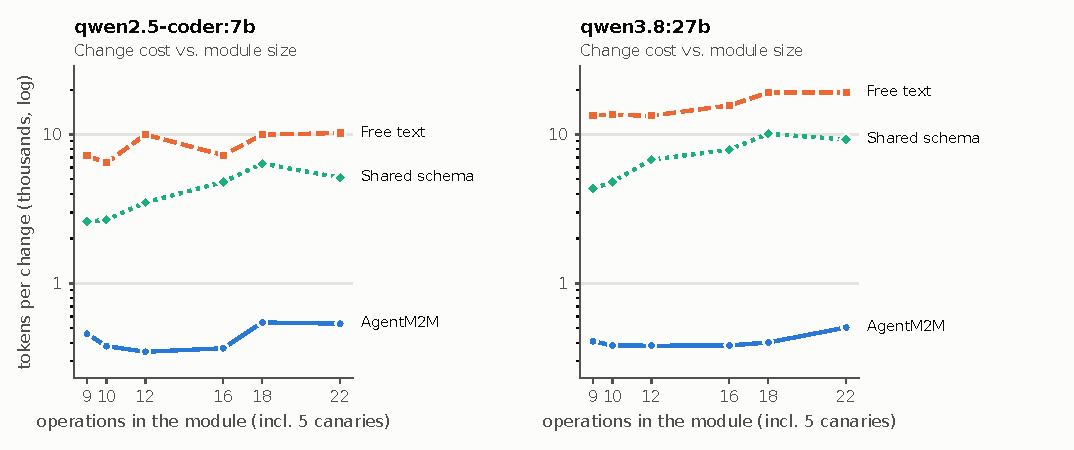
\includegraphics[width=\textwidth]{devbench_two_model_line_change_vs_size.pdf}
\caption{Tokens per change against module size (log scale).}
\label{fig:changesize}
\end{figure}

\noindent\textbf{What we did.} After building, we made three edits to each
repository's requirements and measured the tokens each configuration needed
to bring its code and tests up to date. Free text and shared schema have no
way to update only part of their output, so they must run their pipeline
again. \tool{} re-runs its hand-offs, and the engine calls the LLM only for
bindings whose footprint changed.

\noindent\textbf{How to read it.} The scale is logarithmic because the values
differ by more than ten times: the step from 1 to 10 is as long as the step
from 10 to 100. Dots further left (\Cref{fig:change}) and lines further down
(\Cref{fig:changesize}) are cheaper.

\noindent\textbf{What we see.} \tool{}'s dots sit on the far left, at 0.3 to
0.7 thousand tokens per change, on every repository and with both models.
Free text needs 6.5k--11.2k (small model) and 12.4k--19.9k (large model), and
shared schema 2.0k--6.4k and 3.6k--10.8k. On average a change costs \tool{}
19 and 38 times less than free text, and 9 and 17 times less than shared
schema. In \Cref{fig:changesize}, \tool{}'s line stays flat as modules grow,
while the baselines' lines rise.

\noindent\textbf{Why.} A change touches one operation, so \tool{} re-samples
exactly the bindings of that operation: its signature, its body and its
oracle for a tightened criterion (about 0.8k tokens), the same three for a new
operation (0.48k), and nothing at all for a removal, which the engine
handles by deleting elements. That amount does not depend on how big the
rest of the module is. The baselines regenerate everything, so their cost
grows with the module.

\subsection{Change impact: does each approach know what a change affects?}

\begin{figure}[!htbp]
\centering
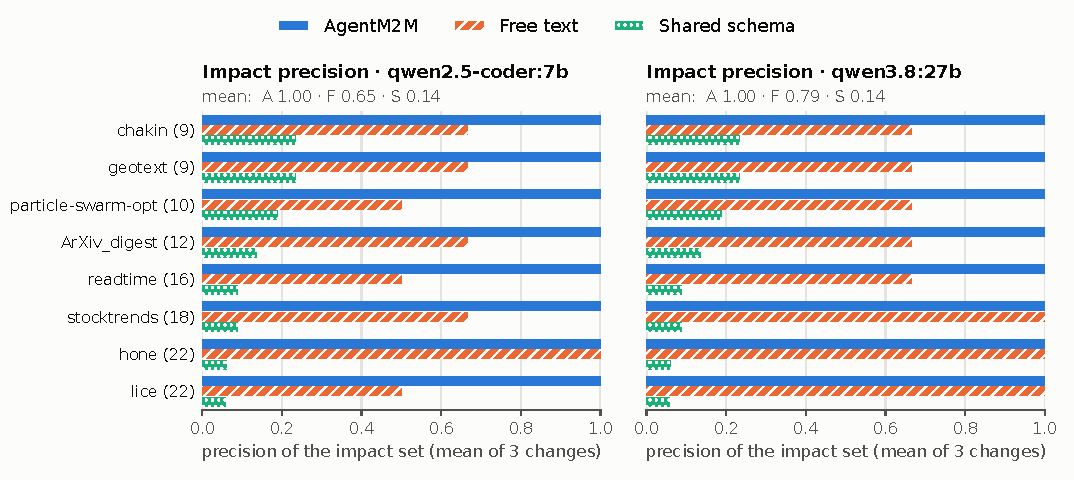
\includegraphics[width=\textwidth]{devbench_two_model_precision.pdf}
\caption{Precision of the predicted impact set: the share of operations a
configuration said were affected that really were. Mean of three changes.}
\label{fig:precision}
\end{figure}

\noindent\textbf{What we did.} For each change, the right answer is exactly
one operation. We compared it with what each configuration said was
affected. \tool{} reads this off its run report (which targets were created,
deleted or re-sampled); free text is asked in one short LLM call; shared
schema, having one undivided document, always says ``everything''.

\noindent\textbf{How to read it.} Precision 1.0 means everything it named was
really affected. Lower means it named operations that were not affected,
which is extra work. Recall, the share of truly affected operations that
were named, is in \Cref{tab:final}.

\noindent\textbf{What we see.} \tool{} scores 1.0 on every repository with
both models, and its recall is 1.0 too. Shared schema's precision falls as
modules grow, from 0.23 at 9 operations to 0.06 at 22, because naming
everything becomes more wrong the more there is. Free text lands between
0.5 and 1.0, and it also missed changes: its recall is 0.75 and 0.79.

\noindent\textbf{Why.} \tool{}'s answer is not a guess. Each binding's
version stamp is a digest of exactly the data it read, so the engine knows
which bindings a changed sentence invalidates (\Cref{sec:step6}). Because
this follows from the rules, it is the same for both models.

\subsection{Putting build and change together}

\begin{figure}[!htbp]
\centering
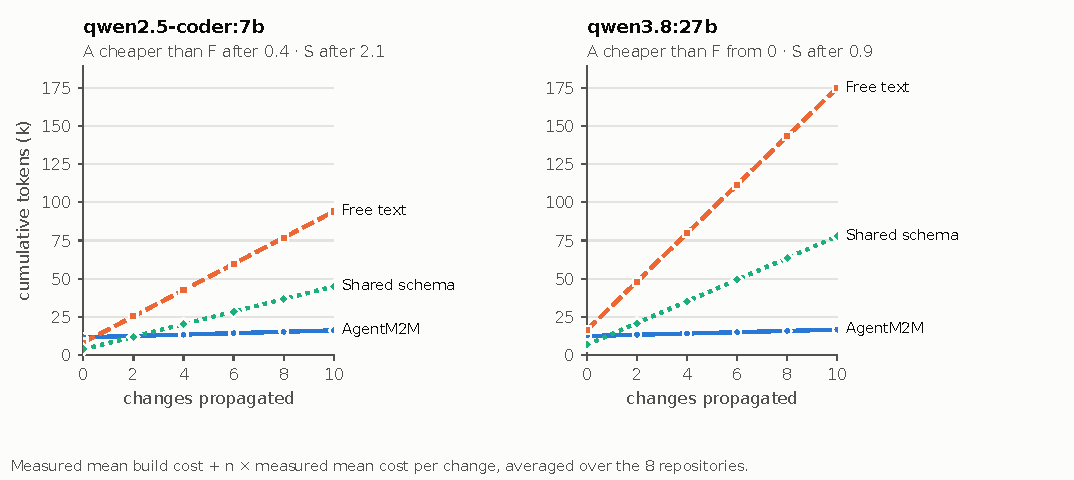
\includegraphics[width=\textwidth]{devbench_two_model_line_cumulative.pdf}
\caption{Total tokens after building once and then propagating $n$ changes:
measured mean build cost plus $n$ times the measured mean cost per change,
averaged over the 8 repositories.}
\label{fig:cumulative}
\end{figure}

\noindent\textbf{What we did.} A real project is built once and then changed
many times. \Cref{fig:cumulative} adds the two measured costs: the line starts
at the build cost ($n=0$) and rises by the cost of one change per step.

\noindent\textbf{How to read it.} Where \tool{}'s line crosses below another
line, its higher build cost has been paid back. The subtitle gives the
crossing point.

\noindent\textbf{What we see.} With the small model, \tool{} starts higher
than free text and shared schema, but its line is almost flat. It is
cheaper than free text from the first change on, and cheaper than shared
schema from the third. With the large model, it is cheaper than free text
from the start, and cheaper than shared schema from the first change. After
ten changes, \tool{} has spent about 16k tokens in total, against about 94k
(small model) and 175k (large model) for free text.

\noindent\textbf{Why.} This combines the two earlier findings: a build cost
that is higher, or similar, and a change cost that is 19--38 times lower. The
more a team changes its requirements, the larger the saving.

\subsection{Adding an agent at runtime}

We added a Security Reviewer to the finished team through a higher-order
transformation (\Cref{sec:hot}). With both models it reviewed all 118 existing
operations across the 8 repositories, and the change needed 7 lines of glue
code. The baselines need an estimated 11 hand-written lines per
configuration, and they review only the operations that exist at that moment
(\Cref{tab:final}). No figure is needed here: the result is the same, 100\%,
on every repository with both models, because it follows from the new
hand-off's rule, not from the LLM.

\subsection{Discussion: what the results do and do not show}

\paragraph{What they show.} Handing off \emph{models} instead of free text
kept every stated requirement, and made change both exact and cheap. The
measures that come from the rules (canaries with \tool{}, impact precision
and recall, reviewer coverage, change cost) were practically the same for a
7B code model and a 27B general model. The baselines' results moved a lot
with the model. With the token discipline of \Cref{sec:tokens}, \tool{}'s many
small calls cost about as much as free text's few long ones when building,
and far less when changing.

\paragraph{What they do not show.}
\begin{itemize}[nosep]
\item \textbf{Working code.} No configuration passed DevBench's acceptance
tests. Canaries test whether stated facts survive the hand-offs, not whether
the program is correct. The requirements model gives each operation its
signature hint and short criteria, not the full behaviour described in the
PRD, so the Developer cannot implement, e.g., which cities
\code{GeoText.cities} must return.
\item \textbf{Cheapest build.} Shared schema is always cheaper to build.
\tool{}'s build cost grows with the number of operations, so for a module that
is built once and never changed it can cost more than free text too (with the
small model, on 6 of 8 repositories).
\item \textbf{Generality.} Eight repositories, one run each, and two models
from one family. That makes this a feasibility check, not a statistical
comparison.
\item \textbf{Truncation.} Two baseline modules with the large model were
longer than the 4096-token cap and were cut off. We count their canaries as
lost and mark them; without the cut, free text's canary count on
\texttt{stocktrends} might be higher.
\item \textbf{MAST.} Our automatic MAST annotator, itself an LLM, flagged
very few failure modes in any configuration, and more P2 modes for \tool{}
with the large model. It may not judge \tool{}'s many short per-binding
transcripts the way it judges a conversation, so we do not base any
conclusion on it.
\end{itemize}

% ===========================================================================
\section{What the walkthrough explains about the pilot results}\label{sec:results}
% ===========================================================================

\begin{center}\small
\begin{tabularx}{\textwidth}{@{}l X X@{}}
\toprule
Result (paper, Section~IV) & Where it comes from in this walkthrough & Consequence \\
\midrule
RQ1: 40/40 canaries reached the code with \tool{} on both models (free text 7 and 25, shared schema 0 and 5) & The \code{body} footprint includes the criterion via \code{op.spec} (\Cref{sec:step4-code}); the pre-fix signature-only footprint lost all canaries. & Structure is preserved by construction; content is preserved exactly as far as the footprint declares it. \\
RQ2: precision = recall = 1.00 on all 48 changes & Stamps are content digests of per-story footprints (\Cref{sec:step6}). & Impact follows from the rules, so it is stable across models. \\
RQ3: 118/118 operations covered on both models, 7 vs.\ 11 glue lines per baseline & A new hand-off starts with an empty trace (\Cref{sec:hot}). & Pre-existing work is picked up automatically; later work too. \\
Tokens: build 11.7k and 12.5k (free text 8.3k and 16.5k); per change 0.45k and 0.42k (free text 8.57k and 15.85k) & The token cost equation and its levers (\Cref{sec:tokens}). & Build cost depends on the rules, not the model; changes cost 19--38$\times$ less than free text (\Cref{sec:experiments}). \\
\bottomrule
\end{tabularx}
\end{center}

\paragraph{Limits that remain visible on \texttt{chakin}.}
\begin{itemize}[nosep]
\item Footprints are declared by the rule author. A footprint that is too
small loses information (the pre-fix canaries); one that is too large dilutes
change impact and costs input tokens on every call.
\item \textsc{Lift} is a free-text boundary: whatever the LLM omits when
lifting text into a model is invisible to every check downstream.
\item Validators check form, not meaning: \code{parses()} accepts
\code{search(lang: str) -> Any}, and \code{compiles()} accepted a checksum
function that ignores the criterion.
\item Failure modes rooted in a single agent's reasoning (MAST FM-1.1, 2.2,
2.6) are out of reach of a coordination layer.
\end{itemize}

% ===========================================================================
\appendix
\section{Reproducing the walkthrough}\label{sec:repro}
% ===========================================================================

\begin{lstlisting}[language=bash, style=engine, literate={}]
# Smoke test with a scripted backend, no network:
python -m evaluation.harness.devbench_run_all --llm mock --repos geotext
# The final experiment (Section "The experiments"), one run per model:
REPOS="geotext readtime particle-swarm-optimization stocktrends chakin lice hone ArXiv_digest"
python -m evaluation.harness.devbench_run_all --llm ollama --model qwen2.5-coder:7b --repos $REPOS
python -m evaluation.harness.devbench_run_all --llm ollama --model qwen3.8:27b     --repos $REPOS
# Tables' data and all figures, from the logs:
python -m evaluation.analysis.make_two_model_figures
# Final logs:
evaluation/harness/logs/devbench_rq{1,2,3}_qwen2.5-coder-7b_*.jsonl
evaluation/harness/logs/devbench_rq{1,2,3}_qwen3.8-27b_*.jsonl  # RQ2 in two files (resumed run)
# Pre-fix logs quoted in the walkthrough:
evaluation/harness/logs/archive_pre_fix/devbench_rq{1,2,3}_qwen3-coder-30b_20260928T193321Z.jsonl
\end{lstlisting}

Relevant sources: \file{evaluation/harness/devbench_loader.py} (seeding),
\file{devbench_metamodels.py} (Step~1), \file{devbench_agentm2m_config.py}
(Step~2), \file{devbench_rules/*.agentm2m} (Step~3),
\file{src/agentm2m/engine/executor.py} and \file{binding.py} (Step~4 and the token rules),
\file{evaluation/harness/token_meter.py} (token accounting),
\file{evaluation/analysis/make_two_model_figures.py} (figures and per-repository data),
\file{engine/lift.py} (Step~5), \file{engine/trace.py} and
\file{impact_injector_devbench.py} (Step~6), \file{team/runtime.py}
(Step~7 and fixpoint), \file{team/hot.py} and \file{hot_reviewer_rq3.py}
(HOT).

\bibliographystyle{IEEEtran}
\bibliography{references}

\end{document}
